\documentclass[]{llncs}
\usepackage[english]{babel}
\usepackage[utf8]{inputenc}
\usepackage{xspace}
\usepackage{amsmath,amssymb,amsfonts}
\usepackage[noalgohanging,lined,noend,linesnumbered]{algorithm2e}
\SetAlCapSkip{1.5ex}
\SetAlFnt{\small }
\setlength{\algomargin}{1.3em}
\newlength{\intextsepBKP}
\setlength{\intextsepBKP}{\intextsep}
\SetInd{.1em}{.5em}
\usepackage[inline]{enumitem}
\usepackage{textcomp}
\usepackage{graphicx,tabularx,placeins,multirow}
\usepackage{xcolor}
\usepackage{soul}
\PassOptionsToPackage{hyphens}{url}\usepackage{hyperref}
\hypersetup{colorlinks=true, allcolors=black}
\usepackage{subcaption}

\begin{document}

\title{
  Distributed Novelty Detection at the Edge for IoT Network Security
  \thanks{The authors would like to thank Brazilian funding agencies FAPESP and CNPq for the financial support.}
}
\titlerunning{Distributed ND at the edge for IoT network security}

\author{
  Luís Puhl\inst{1}\orcidID{0000-0003-2118-9992} \and
  Guilherme Weigert Cassales\inst{1}\orcidID{0000-0003-4029-2047} \and
  Helio Crestana Guardia\inst{1}\orcidID{0000-0001-5010-747X} \and
  Hermes Senger\inst{1}\orcidID{0000-0003-1273-9809}
}
\authorrunning{L. Puhl et al.}
\institute{
  Universidade Federal de São Carlos, Brasil\\
  \url{https://www2.ufscar.br/}
}

\maketitle

\newcommand{\refminas}{\textit{Ref}\xspace}
\newcommand{\mfog}{\textit{MFOG}\xspace}
\newcommand{\iot}{IoT\xspace}
\newcommand{\nids}{NIDS\xspace}
\newcommand{\nd}{DSND\xspace}
\newcommand{\minas}{MINAS\xspace}

\begin{abstract}

  The ongoing implementation of the Internet of Things (\iot) is sharply
  increasing the number and variety of small devices on edge networks and,
  following this increase, the attack opportunities for hostile agents also
  increases, requiring more from network administrators and the need for tools
  to detect and react to those threats.
  % 
  One such tool are the Network Intrusion Detection Systems (\nids)
  which captures and analyses network traffic,
  acting when a known attack or a new pattern is detected.
  For a network security tool to operate in the context of edge and
  \iot it has to comply with processing time, storage space and energy
  requirements alongside traditional requirements for stream and network
  analysis like accuracy and scalability.
  % 
  Using a previously defined architecture (IDSA-IoT),
  we address the construction and evaluation of a prototype distributed \nids
  with the Data Stream Novelty Detection algorithm (\nd) MINAS
  employing C and MPI library.
  % 
  We discuss the algorithm steps, how it can be deployed in a distributed
  environment, the impacts on the accuracy and evaluate performance and
  scalability using a cluster of constrained devices commonly found in \iot
  scenarios.
  % 
  % We found an increase of \textit{A 0.0} processed network flow descriptors per
  % core added to the cluster.
  % Also \textit{B 0.0\%} and \textit{C 0.0\%} change in
  % \textit{F1Score} in the tested datasets when stream was unlimited in speed and
  % limited to \textit{0.0 z MB/s} respectively.
  We found a marginal ($2$ to $4\%$) difference in true positive (hits) between
  original, serial and distributed executions, consuming a months worth of flow
  descriptors in $300$ seconds.
\end{abstract}

\ifdefined\IEEEkeywords
\begin{IEEEkeywords}
  % Detecção de Novidades, Detecção de Intrusão, Fluxos de Dados, Computação Distribuı́da, Computação em Névoa, Internet das Coisas.
  novelty detection, intrusion detection, data streams,
  distributed system, edge computing, internet of things
\end{IEEEkeywords}
\else
\keywords{
novelty detection \and intrusion detection \and data streams \and
distributed system \and edge computing \and internet of things
}
\fi

\section{Introduction {\color{red} Nao mexer por enquanto}} 


\newcommand{\refminas}{\textit{Ref}\xspace}
\newcommand{\mfog}{\textit{MFOG}\xspace}
\newcommand{\iot}{IoT\xspace}
\newcommand{\nids}{NIDS\xspace}
\newcommand{\ds}{DS\xspace}

The advent of Internet of Things (IoT)
is growing the count and diversity of
devices on edge networks, this growth increases network traffic patterns and
extends opportunities for cyber attacks presenting new challenges for network
administrators.
To address those challenges new Network Intrusion Detection Systems (NIDS) and
architectures can be explored, especially in Fog Computing and Data Stream (DS)
areas.

% Data Stream (DS)

% - Desafio, resposta, justificativa.
% - Artigo para setembro ou outubro.
% - Revisão dos valores da avaliação.

% ### Desafios, Respostas e Justificativas

% Desafios de arquitetura e validação:

% - Construção de um protótipo da arquitetura IDSA-IoT:
%   - Kafka (Python): Distribuição e balanceamento pelo cluster kafka, hipótese refutada.
%   - Flink (Java ou Scala): Execução do cluster nos dispositivos de névoa, hipótese refutada.
%   - MPI (C e Python): Execução do cluster nos dispositivos de névoa, hipótese aceita.
% - Reimplementação do algoritmo MINAS com fidelidade:
%   - Duas versões: a descrita e a implementação de referência (em Java).
%   - Resolução: utilizar a descrição, não *seguir* a imp. referência, apenas como ponto de comparação. Exemplos:
%     - Definição de raio `r = f * σ` (fator vezes desvio padrão) para `r = max(distance)` (distância máxima);
%     - Tamanho do buffer de desconhecidos e frequência de execução do passo de detecção de novidade;

\begin{highlight}
Expected results:
A system that embraces and explores the inherent distribution of fog computing
in a IoT scenario opposing regular systems where data streams are collected and
centralized before processing;
Impact assessment of the impact of distributed, regional flow characteristics,
local vs global vs distributed forgetting mechanism and other polices.

IDS characteristics and description of physical scenario.

MINAS characteristics.

Distribution and IDSA-IoT architecture.
\end{highlight}

This paper is structured as follows:
Section \ref{sec:related} presents previous works that addresses related
problems and how they influenced our solution.
Section \ref{sec:implementation} address our proposal, the work done, issues
found during implementation and discusses parameters and configurations options
and how we arrived at our choices.
Section \ref{sec:experiments} shows experiments layouts and results, we
compare serial and distributed implementation's metrics for validation,
we also evaluate communication delay effects on classification metrics and
conclude with the speedup per core and overall maximum stream speed.
Section \ref{sec:conclusion} summarizes the research results and presents our
final conclusions and future works.

\section{MINAS}
\label{sec:minas}

%  ******************* Texto quali ************************
% \subsection{O Algoritmo MINAS}
% Apresentar o MINAS de forma resumida (1 pagina no max): como funciona, etc. 



MINAS is an offline-online clustering algorithm, which means it has two distinct phases.
The first phase generates the model by creating several micro-clusters based
on a separate training set that is processed offline.
Each micro-cluster can be associated with only one class of the problem,
but each class can have many micro-clusters.
The online phase is where the model performs three tasks in (near) real-time.
% Our proposal focuses on the online phase, therefore we will describe it in more detail.
We describe the online phase in more detail since we focus on its tasks. 

In summary, MINAS executes the classification, novelty detection,
and model update tasks in the online phase.

% ******************* OLD ******************* 
% % classification
% For each arriving instance, the model tries to explain (i.e, classify) the instance by associating it with an existing micro-cluster. 
% % update
% If there is a micro-cluster within a parameterizable distance of the instance, the instance is grouped in that micro-cluster  by adding (i.e., updating) its attributes to the micro-cluster's feature vector. 
% % temp memory + ND
% Otherwise, this instance will be considered unknown and saved on a temporary memory for future use. 
% When the size of the temporary memory reaches a parameterizable value MINAS stops classifying new instances and performs the novelty detection process. 
% The novelty detection tries to find 
% % linha abaixo pode ser omitida se achar melhor
% valid and representative (i.e., \textit{silhouette} > 0 and at least a parameterizable number of instances) 
% groups of unknown instances from the temporary memory.
% Each 
% % linha abaixo pode ser omitida se achar melhor
% % valid and representative
% group found can be a new pattern if the distance between it and its closest micro-cluster is bigger than a parameterizable threshold or, otherwise, an extension of said micro-cluster.
% ******************* NEW ******************* 
MINAS tries to classify each incoming unlabeled instance according to the
current decision model. Instances unexplained by the model
% pode descomentar linha abaixo para dar mais "detalhes"
% (i.e., distance from all existing micro-clusters bigger than a parameterizable threshold)
receive an \textit{unknown} label and are stored in temporary memory for future
analysis.
When this temporary memory reaches a parameterizable size, MINAS groups the
instances to form new micro-clusters.
Each micro-cluster is validated to discard the non-cohesive or unrepresentative
ones.
Valid micro-clusters are analyzed to decide if they represent an extension of a
known pattern or a completely new pattern. In both cases, the model absorbs the
valid micro-clusters and starts using them to classify new instances.
MINAS also has a mechanism to forget micro-clusters that became obsolete and
unrepresentative of the current data stream distribution.
Besides, MINAS also cleans the temporary memory to eliminate ungrouped unknown
instances as they represent noise~\cite{Faria2016minas}.

% Citar que o trabalho anterior já validou o uso do MINAs para detecção de novidade porem com uma implementação sequencial. 

Authors in~\cite{Cassales2019a} validated the usage of the MINAS algorithm for
the Intrusion Detection and deploying it on edge. However, they used the
sequential version of the algorithm, where classification stops completely to
execute novelty detection.

% Figura do MINAS (offline + online) ...
% \todo[inline, color=brown]{\textbf{Guilherme:} Não coloquei figura porque as figuras originais do MINAS ocupam bastante espaço (https://sci-hub.se/10.1007/s10618-015-0433-y pg 9) e a do MFog está mais completa.}

% Formally, a data stream $S$ is a massive sequence of data elements
% $x_1, x_2, \dots, x_n$ that is, $S={\{x_i\}}_{i=1}^n$, which is potentially
% unbounded (n → $\infty$).
% Compared to traditional (batch) data mining, stream processing algorithms have
% additional requirements.
% For instance, with a potentially infinite data stream, storing data for late
% processing is not a choice due to memory constraints.
% Algorithms need to incrementally process incoming data instances in a single
% pass while operating under memory and response time constraints.
% Furthermore, as data streams present transient behavior, prediction models often
% need to be incremented to adapt to concept drift observed in data.



% \begin{algorithm}
%     \DontPrintSemicolon
%     \SetKwFunction{FMain}{Main}
%     \SetKwProg{Fn}{algorithm}{:}{}
%     \Fn{\FMain{$f$, $a$, $b$, $\varepsilon$}}{
%           a\;
%           b\;
%           \KwRet\;
%     }
%     \;
%     \SetKwProg{Pn}{algorithm}{:}{\KwRet}
%     \Pn{\FMain{$f$, $a$, $b$, $\varepsilon$}}{
%           a\;
%           b\;
%     }
% \end{algorithm}
% \IncMargin{1em}
\begin{algorithm}[h]
% \begin{multicols}{2}
    \SetKwProg{KwFunction}{algorithm}{:}{}
    % \DontPrintSemicolon
    % \KwIn{sample, ModelSet, params as p}
    % \KwOut{Classified Sample}
    % 
    \SetKwData{CW}{cleaningWindow}
    \SetKwData{NDT}{noveltyDetectionTrigger}
    \SetKwData{MEPC}{minExamplesPerCluster}
    \SetKwData{NF}{noveltyFactor}
    % 
    % \KwSty{Parameters}: cleaningWindow as \CW,
    % noveltyDetectionTrigger as \NDT,
    % minExamplesPerCluster as \MEPC,
    % noveltyFactor as \NF\\
    % 
    \SetKwFunction{nearestCluster}{nearestCluster}
    \SetKwFunction{clustering}{clustering}
    \SetKwFunction{sizeOf}{sizeOf}
    \SetKwFunction{NoveltyDetection}{NoveltyDetection}
    \SetKwFunction{handleModelSleep}{moveToSleep}
    \SetKwFunction{removeOldSamples}{removeOldSamples}
    % 
    % \KwData{ UnkownSet $\leftarrow$ $\emptyset$, ModelSleepSet $\leftarrow$ $\emptyset$, lastCleanupTime $\leftarrow$ now() }
    % 
    \KwFunction{\NoveltyDetection{Model, Samples}}{
        newModelSet $\leftarrow$ $\emptyset$\;
        \ForEach{cl in \clustering(Samples)}{
            \If{$|cl.sampleSet| \geq$ \MEPC}{
                (distance, near) $\leftarrow$ \nearestCluster(cl, Model)\;
                \eIf{distance $<$ near.radius $\times$ \NF}{
                    cl.label $\leftarrow$ near.label\;
                    cl.type $\leftarrow$ extension\;
                }{
                    cl.label $\leftarrow$ noveltyIndex\;
                    noveltyIndex $\leftarrow$ noveltyIndex $+ 1$\;
                    cl.type $\leftarrow$ novelty\;
                }
                Samples $\leftarrow$ Samples $\ominus$ cl.sampleSet\;
                newModelSet $\leftarrow$ newModelSet $\oplus$ cl\;
            }
        }
        \Return{newModelSet}
    }
    \label{alg:MINAS-nd}
    \caption{Minas: Novelty Detection task.}
\end{algorithm}
\begin{algorithm}
    \SetKwProg{KwFunction}{algorithm}{:}{}
    % \DontPrintSemicolon
    % \KwIn{sample, ModelSet, params as p}
    % \KwOut{Classified Sample}
    % 
    \SetKwData{CW}{cleaningWindow}
    \SetKwData{NDT}{noveltyDetectionTrigger}
    \SetKwData{MEPC}{minExamplesPerCluster}
    \SetKwData{NF}{noveltyFactor}
    % 
    % \KwSty{Parameters}: cleaningWindow as \CW,
    % noveltyDetectionTrigger as \NDT,
    % minExamplesPerCluster as \MEPC,
    % noveltyFactor as \NF\\
    % 
    \SetKwFunction{nearestCluster}{nearestCluster}
    \SetKwFunction{clustering}{clustering}
    \SetKwFunction{sizeOf}{sizeOf}
    \SetKwFunction{NoveltyDetection}{NoveltyDetection}
    \SetKwFunction{handleModelSleep}{moveToSleep}
    \SetKwFunction{removeOldSamples}{removeOldSamples}
    % 
    \SetKwProg{algorithm}{algorithm}{:}{}
    \SetKwFor{With}{with}{}{}
    \SetKw{continue}{continue}
    % 
    \SetKwData{CW}{CW}
    \SetKwData{noveltyDetectionTrigger}{NDT}
    \SetKwData{MEPC}{MEPC}
    \SetKwData{NF}{NF}
    \SetKwData{mpiSize}{mpiSize}
    \SetKwData{mpiRank}{mpiRank}
    \SetKwData{EndOfStream}{EndOfStream}
    % 
    \KwIn{ModelSet, Sample Stream}
    \KwOut{Classified Stream as $out$}
    \SetKwFunction{MinasOnline}{MinasOnline}
    \KwFunction{\MinasOnline{ModelSet, SampleStream}}{
        UnkownSet $\leftarrow$ $\emptyset$, ModelSleepSet $\leftarrow$ $\emptyset$ \;
        lastCleanup $\leftarrow 0$ , noveltyIndex $\leftarrow 0$\;
        % sampleIn $\leftarrow 0$\;
        \ForEach{ {$sample_{i}$} $\in$ SampleStream }{
            % sample.label $\leftarrow$ unknown\;
            % (distance, cluster) $\leftarrow$ \nearestCluster(sample, ModelSet)\;
            nearest $\leftarrow$ \nearestCluster(sample, ModelSet)\;
            \eIf{nearest.distance $<$ nearest.cluster.radius}{
                sample.label $\leftarrow$ nearest.cluster.label\;
                nearest.cluster.lastUsed $ \leftarrow i $ \;
                % $out \leftarrow$ sample\;
                % outputStream.append(sample);
                % \textbf{continue};
                % \Return sample\;
            }
            {
                sample.label $\leftarrow$ unknown\;
                UnkownSet $\leftarrow$ UnkownSet $\cup$ sample\;
                \If{$|UnkownSet| \geq$ \NDT}{
                    % \tcc{Novelty Detection}
                    novelties $\leftarrow$ \NoveltyDetection(ModelSet $\cup$ ModelSleepSet, *UnkownSet)\;
                    ModelSet $\leftarrow$ ModelSet $\cup$ novelties\;
                }
                \If{ $ i > $ ( lastCleanup $ + $ \CW )}{
                    ModelSet $\leftarrow$ \handleModelSleep(ModelSet, *ModelSleepSet, lastCleanup)\;
                    UnkownSet $\leftarrow$ \removeOldSamples(UnkownSet, lastCleanup)\;
                    lastCleanup $ \leftarrow i $\;
                }
                % \Return sample\;
            }
            outputStream.append(sample);
            % $out \leftarrow$ sample\;
        }
    }
% \end{multicols}
% }
\label{alg:MINAS}
\caption{Our interpretation of MINAS \cite{faria2013novelty,Faria2016minas,Cassales2019a}}
\end{algorithm}
% \DecMargin{1em}


% --------------------------------------------------------------------------------------------------

% \begin{algorithm}[ht]
%   \caption{MINAS \cite{Faria2016minas,Cassales2019a}}
%   \label{alg:MINAS}
%   \renewcommand{\algorithmicrequire}{\textbf{Entrada:}}
%   \begin{algorithmic}[1]
%     %T $\leftarrow$ limiar de distância para pertencer ao grupo
%     %P $\leftarrow$ tempo de "inatividade" para passar para memória sleep
%     %ts $\leftarrow$ limiar para remoção de exemplos da memória temporária
%     \REQUIRE $Modelo,FCD,T,NumMinExemplos,ts,P$
%     \STATE $MemTmp \leftarrow \emptyset$
%     \STATE $MemSleep \leftarrow \emptyset$
%     \FORALL{$exemplo \in FCD$}
%     \STATE $(Dist,micro) \leftarrow$ micro-mais-proximo($exemplo,Modelo$)
%     \IF{$Dist < $ raio($micro$)}
%     \STATE $exemplo.classe \leftarrow micro.rotulo$
%     \STATE atualizar-micro($micro,exemplo$)
%     \ELSE
%     \STATE $exemplo.classe \leftarrow desconhecido$
%     \STATE $MemTmp \leftarrow MemTmp \cup exemplo$
%     \IF{$|MemTmp| \geq NumMinExemplos$}
%     \STATE $Modelo \leftarrow $ deteccao-novidade($Modelo,MemTmp,T$)
%     \ENDIF
%     \ENDIF
%     \STATE $TempoAtual \leftarrow exemplo.T$
%     \IF{$TempoAtual$ mod $TamJanela == 0$}
%     \STATE $Modelo \leftarrow$ mover-micro-grupos-mem-sleep($Modelo,MemSleep,P$)
%     \STATE $MemTmp \leftarrow$ remover-exemplos-antigos($MemTmp,ts$)
%     \ENDIF
%     \ENDFOR
%   \end{algorithmic}
% \end{algorithm}

% \begin{algorithm}[ht]
%   \caption{MINAS \cite{Faria2016minas,Cassales2019a}}
%   \label{alg:MINAS}
%   \renewcommand{\algorithmicrequire}{\textbf{Entrada:}}
%   \begin{algorithmic}[1]
%   \IF{root}
%     \WHILE{true}
%     \IF{can_read(S)}
%     input(S, $s$)
%     send(s, i++)
%     \ENDIF
%     \IF{can_rcv($(s, l)$, any)}
%         output($(s, l)$)
%         \IF{$l == '-'$ )}
%             store($(s, l)$, unknowns)
%             % \IF{$|MemTmp| \geq NumMinExemplos$}
%             % \STATE $Modelo \leftarrow $ deteccao-novidade($Modelo,MemTmp,T$)
%             % \ENDIF
%             % \ENDIF
%             % \STATE $TempoAtual \leftarrow exemplo.T$
%             % \IF{$TempoAtual$ mod $TamJanela == 0$}
%             % \STATE $Modelo \leftarrow$ mover-micro-grupos-mem-sleep($Modelo,MemSleep,P$)
%             % \STATE $MemTmp \leftarrow$ remover-exemplos-antigos($MemTmp,ts$)
%             % \ENDIF
%         \ENDIF
%     \ENDIF
%   \ENDWHILE
%   \ENDIF
%   \IF{leaf}
%     rcv($s$, root)
%     $l$ $\leftarrow$ classify($s$)
%     send($(s, l)$, root)
%   \ENDIF
%   \end{algorithmic}
% \end{algorithm}

% \begin{algorithm}
%   \caption{High level parallel algorithm}
%   \label{alg:highlevel-new}
%   \begin{algorithmic}[1]
%     \State {\bf Input}: an ensemble $E$, $num\_threads$, a data stream $S$
%     \State $P \gets Create\_service\_thread\_pool(num\_threads)$
%     \State $T \gets Create\_trainers\_collection(E)$
%     \For {each arriving instance $I$ in stream $S$}
%     \State $E$.classify($I$)
%     \For  {each trainer $T_i$ in trainers $T$} 
%     \State $k \gets poisson(\lambda)$
%     \State $T_i.update(I, k)$
%     \EndFor
%     \For {all trainers $T$} {\bf in parallel}
%     \State $W\_inst \gets I * k$
%     \State $Train\_on\_instance(W\_inst)$
%     \EndFor
%     \If {change detected}
%     \State $reset\_classifier$
%     \EndIf
%     \EndFor
%   \end{algorithmic}
% \end{algorithm}



% \begin{figure}[ht]
% \subfloat[float]{
% \begin{minipage}[c][1\width]{0.5\textwidth}
%     \begin{algorithm}[h]
%     % {\tiny 
% \begin{algorithm}
%     \DontPrintSemicolon
%     \SetKwFunction{FMain}{Main}
%     \SetKwProg{Fn}{algorithm}{:}{}
%     \Fn{\FMain{$f$, $a$, $b$, $\varepsilon$}}{
%           a\;
%           b\;
%           \KwRet\;
%     }
%     \;
%     \SetKwProg{Pn}{algorithm}{:}{\KwRet}
%     \Pn{\FMain{$f$, $a$, $b$, $\varepsilon$}}{
%           a\;
%           b\;
%     }
% \end{algorithm}
% \IncMargin{1em}
\begin{algorithm}[h]
% \begin{multicols}{2}
    \SetKwProg{KwFunction}{algorithm}{:}{}
    % \DontPrintSemicolon
    % \KwIn{sample, ModelSet, params as p}
    % \KwOut{Classified Sample}
    % 
    \SetKwData{CW}{cleaningWindow}
    \SetKwData{NDT}{noveltyDetectionTrigger}
    \SetKwData{MEPC}{minExamplesPerCluster}
    \SetKwData{NF}{noveltyFactor}
    % 
    % \KwSty{Parameters}: cleaningWindow as \CW,
    % noveltyDetectionTrigger as \NDT,
    % minExamplesPerCluster as \MEPC,
    % noveltyFactor as \NF\\
    % 
    \SetKwFunction{nearestCluster}{nearestCluster}
    \SetKwFunction{clustering}{clustering}
    \SetKwFunction{sizeOf}{sizeOf}
    \SetKwFunction{NoveltyDetection}{NoveltyDetection}
    \SetKwFunction{handleModelSleep}{moveToSleep}
    \SetKwFunction{removeOldSamples}{removeOldSamples}
    % 
    % \KwData{ UnkownSet $\leftarrow$ $\emptyset$, ModelSleepSet $\leftarrow$ $\emptyset$, lastCleanupTime $\leftarrow$ now() }
    % 
    \KwFunction{\NoveltyDetection{Model, Samples}}{
        newModelSet $\leftarrow$ $\emptyset$\;
        \ForEach{cl in \clustering(Samples)}{
            \If{$|cl.sampleSet| \geq$ \MEPC}{
                (distance, near) $\leftarrow$ \nearestCluster(cl, Model)\;
                \eIf{distance $<$ near.radius $\times$ \NF}{
                    cl.label $\leftarrow$ near.label\;
                    cl.type $\leftarrow$ extension\;
                }{
                    cl.label $\leftarrow$ noveltyIndex\;
                    noveltyIndex $\leftarrow$ noveltyIndex $+ 1$\;
                    cl.type $\leftarrow$ novelty\;
                }
                Samples $\leftarrow$ Samples $\ominus$ cl.sampleSet\;
                newModelSet $\leftarrow$ newModelSet $\oplus$ cl\;
            }
        }
        \Return{newModelSet}
    }
    \label{alg:MINAS-nd}
    \caption{Minas: Novelty Detection task.}
\end{algorithm}
\begin{algorithm}
    \SetKwProg{KwFunction}{algorithm}{:}{}
    % \DontPrintSemicolon
    % \KwIn{sample, ModelSet, params as p}
    % \KwOut{Classified Sample}
    % 
    \SetKwData{CW}{cleaningWindow}
    \SetKwData{NDT}{noveltyDetectionTrigger}
    \SetKwData{MEPC}{minExamplesPerCluster}
    \SetKwData{NF}{noveltyFactor}
    % 
    % \KwSty{Parameters}: cleaningWindow as \CW,
    % noveltyDetectionTrigger as \NDT,
    % minExamplesPerCluster as \MEPC,
    % noveltyFactor as \NF\\
    % 
    \SetKwFunction{nearestCluster}{nearestCluster}
    \SetKwFunction{clustering}{clustering}
    \SetKwFunction{sizeOf}{sizeOf}
    \SetKwFunction{NoveltyDetection}{NoveltyDetection}
    \SetKwFunction{handleModelSleep}{moveToSleep}
    \SetKwFunction{removeOldSamples}{removeOldSamples}
    % 
    \SetKwProg{algorithm}{algorithm}{:}{}
    \SetKwFor{With}{with}{}{}
    \SetKw{continue}{continue}
    % 
    \SetKwData{CW}{CW}
    \SetKwData{noveltyDetectionTrigger}{NDT}
    \SetKwData{MEPC}{MEPC}
    \SetKwData{NF}{NF}
    \SetKwData{mpiSize}{mpiSize}
    \SetKwData{mpiRank}{mpiRank}
    \SetKwData{EndOfStream}{EndOfStream}
    % 
    \KwIn{ModelSet, Sample Stream}
    \KwOut{Classified Stream as $out$}
    \SetKwFunction{MinasOnline}{MinasOnline}
    \KwFunction{\MinasOnline{ModelSet, SampleStream}}{
        UnkownSet $\leftarrow$ $\emptyset$, ModelSleepSet $\leftarrow$ $\emptyset$ \;
        lastCleanup $\leftarrow 0$ , noveltyIndex $\leftarrow 0$\;
        % sampleIn $\leftarrow 0$\;
        \ForEach{ {$sample_{i}$} $\in$ SampleStream }{
            % sample.label $\leftarrow$ unknown\;
            % (distance, cluster) $\leftarrow$ \nearestCluster(sample, ModelSet)\;
            nearest $\leftarrow$ \nearestCluster(sample, ModelSet)\;
            \eIf{nearest.distance $<$ nearest.cluster.radius}{
                sample.label $\leftarrow$ nearest.cluster.label\;
                nearest.cluster.lastUsed $ \leftarrow i $ \;
                % $out \leftarrow$ sample\;
                % outputStream.append(sample);
                % \textbf{continue};
                % \Return sample\;
            }
            {
                sample.label $\leftarrow$ unknown\;
                UnkownSet $\leftarrow$ UnkownSet $\cup$ sample\;
                \If{$|UnkownSet| \geq$ \NDT}{
                    % \tcc{Novelty Detection}
                    novelties $\leftarrow$ \NoveltyDetection(ModelSet $\cup$ ModelSleepSet, *UnkownSet)\;
                    ModelSet $\leftarrow$ ModelSet $\cup$ novelties\;
                }
                \If{ $ i > $ ( lastCleanup $ + $ \CW )}{
                    ModelSet $\leftarrow$ \handleModelSleep(ModelSet, *ModelSleepSet, lastCleanup)\;
                    UnkownSet $\leftarrow$ \removeOldSamples(UnkownSet, lastCleanup)\;
                    lastCleanup $ \leftarrow i $\;
                }
                % \Return sample\;
            }
            outputStream.append(sample);
            % $out \leftarrow$ sample\;
        }
    }
% \end{multicols}
% }
\label{alg:MINAS}
\caption{Our interpretation of MINAS \cite{faria2013novelty,Faria2016minas,Cassales2019a}}
\end{algorithm}
% \DecMargin{1em}


% --------------------------------------------------------------------------------------------------

% \begin{algorithm}[ht]
%   \caption{MINAS \cite{Faria2016minas,Cassales2019a}}
%   \label{alg:MINAS}
%   \renewcommand{\algorithmicrequire}{\textbf{Entrada:}}
%   \begin{algorithmic}[1]
%     %T $\leftarrow$ limiar de distância para pertencer ao grupo
%     %P $\leftarrow$ tempo de "inatividade" para passar para memória sleep
%     %ts $\leftarrow$ limiar para remoção de exemplos da memória temporária
%     \REQUIRE $Modelo,FCD,T,NumMinExemplos,ts,P$
%     \STATE $MemTmp \leftarrow \emptyset$
%     \STATE $MemSleep \leftarrow \emptyset$
%     \FORALL{$exemplo \in FCD$}
%     \STATE $(Dist,micro) \leftarrow$ micro-mais-proximo($exemplo,Modelo$)
%     \IF{$Dist < $ raio($micro$)}
%     \STATE $exemplo.classe \leftarrow micro.rotulo$
%     \STATE atualizar-micro($micro,exemplo$)
%     \ELSE
%     \STATE $exemplo.classe \leftarrow desconhecido$
%     \STATE $MemTmp \leftarrow MemTmp \cup exemplo$
%     \IF{$|MemTmp| \geq NumMinExemplos$}
%     \STATE $Modelo \leftarrow $ deteccao-novidade($Modelo,MemTmp,T$)
%     \ENDIF
%     \ENDIF
%     \STATE $TempoAtual \leftarrow exemplo.T$
%     \IF{$TempoAtual$ mod $TamJanela == 0$}
%     \STATE $Modelo \leftarrow$ mover-micro-grupos-mem-sleep($Modelo,MemSleep,P$)
%     \STATE $MemTmp \leftarrow$ remover-exemplos-antigos($MemTmp,ts$)
%     \ENDIF
%     \ENDFOR
%   \end{algorithmic}
% \end{algorithm}

% \begin{algorithm}[ht]
%   \caption{MINAS \cite{Faria2016minas,Cassales2019a}}
%   \label{alg:MINAS}
%   \renewcommand{\algorithmicrequire}{\textbf{Entrada:}}
%   \begin{algorithmic}[1]
%   \IF{root}
%     \WHILE{true}
%     \IF{can_read(S)}
%     input(S, $s$)
%     send(s, i++)
%     \ENDIF
%     \IF{can_rcv($(s, l)$, any)}
%         output($(s, l)$)
%         \IF{$l == '-'$ )}
%             store($(s, l)$, unknowns)
%             % \IF{$|MemTmp| \geq NumMinExemplos$}
%             % \STATE $Modelo \leftarrow $ deteccao-novidade($Modelo,MemTmp,T$)
%             % \ENDIF
%             % \ENDIF
%             % \STATE $TempoAtual \leftarrow exemplo.T$
%             % \IF{$TempoAtual$ mod $TamJanela == 0$}
%             % \STATE $Modelo \leftarrow$ mover-micro-grupos-mem-sleep($Modelo,MemSleep,P$)
%             % \STATE $MemTmp \leftarrow$ remover-exemplos-antigos($MemTmp,ts$)
%             % \ENDIF
%         \ENDIF
%     \ENDIF
%   \ENDWHILE
%   \ENDIF
%   \IF{leaf}
%     rcv($s$, root)
%     $l$ $\leftarrow$ classify($s$)
%     send($(s, l)$, root)
%   \ENDIF
%   \end{algorithmic}
% \end{algorithm}

% \begin{algorithm}
%   \caption{High level parallel algorithm}
%   \label{alg:highlevel-new}
%   \begin{algorithmic}[1]
%     \State {\bf Input}: an ensemble $E$, $num\_threads$, a data stream $S$
%     \State $P \gets Create\_service\_thread\_pool(num\_threads)$
%     \State $T \gets Create\_trainers\_collection(E)$
%     \For {each arriving instance $I$ in stream $S$}
%     \State $E$.classify($I$)
%     \For  {each trainer $T_i$ in trainers $T$} 
%     \State $k \gets poisson(\lambda)$
%     \State $T_i.update(I, k)$
%     \EndFor
%     \For {all trainers $T$} {\bf in parallel}
%     \State $W\_inst \gets I * k$
%     \State $Train\_on\_instance(W\_inst)$
%     \EndFor
%     \If {change detected}
%     \State $reset\_classifier$
%     \EndIf
%     \EndFor
%   \end{algorithmic}
% \end{algorithm}

 }
%     \SetAlgoVlined
%     \KwIn{sample, ModelSet, params as p}
%     \label{alg:MINAS}
%     \caption{Our interpretation of MINAS \cite{faria2013novelty,Faria2016minas,Cassales2019a}}
%     \end{algorithm}
% \hfill 
% \end{minipage}}
% \end{figure}

% \begin{tabular}{cc}
%     asasdfad
%     % \includegraphics[width=0.4\textwidth]{figures/cassalesimgs-000.png}
%     &
%     asdfasdfa
%     % \includegraphics[width=0.4\textwidth]{figures/cassalesimgs-000.png}
% \end{tabular}


% {\begin{algorithm}[h]
% {\tiny 
% \begin{algorithm}
%     \DontPrintSemicolon
%     \SetKwFunction{FMain}{Main}
%     \SetKwProg{Fn}{algorithm}{:}{}
%     \Fn{\FMain{$f$, $a$, $b$, $\varepsilon$}}{
%           a\;
%           b\;
%           \KwRet\;
%     }
%     \;
%     \SetKwProg{Pn}{algorithm}{:}{\KwRet}
%     \Pn{\FMain{$f$, $a$, $b$, $\varepsilon$}}{
%           a\;
%           b\;
%     }
% \end{algorithm}
% \IncMargin{1em}
\begin{algorithm}[h]
% \begin{multicols}{2}
    \SetKwProg{KwFunction}{algorithm}{:}{}
    % \DontPrintSemicolon
    % \KwIn{sample, ModelSet, params as p}
    % \KwOut{Classified Sample}
    % 
    \SetKwData{CW}{cleaningWindow}
    \SetKwData{NDT}{noveltyDetectionTrigger}
    \SetKwData{MEPC}{minExamplesPerCluster}
    \SetKwData{NF}{noveltyFactor}
    % 
    % \KwSty{Parameters}: cleaningWindow as \CW,
    % noveltyDetectionTrigger as \NDT,
    % minExamplesPerCluster as \MEPC,
    % noveltyFactor as \NF\\
    % 
    \SetKwFunction{nearestCluster}{nearestCluster}
    \SetKwFunction{clustering}{clustering}
    \SetKwFunction{sizeOf}{sizeOf}
    \SetKwFunction{NoveltyDetection}{NoveltyDetection}
    \SetKwFunction{handleModelSleep}{moveToSleep}
    \SetKwFunction{removeOldSamples}{removeOldSamples}
    % 
    % \KwData{ UnkownSet $\leftarrow$ $\emptyset$, ModelSleepSet $\leftarrow$ $\emptyset$, lastCleanupTime $\leftarrow$ now() }
    % 
    \KwFunction{\NoveltyDetection{Model, Samples}}{
        newModelSet $\leftarrow$ $\emptyset$\;
        \ForEach{cl in \clustering(Samples)}{
            \If{$|cl.sampleSet| \geq$ \MEPC}{
                (distance, near) $\leftarrow$ \nearestCluster(cl, Model)\;
                \eIf{distance $<$ near.radius $\times$ \NF}{
                    cl.label $\leftarrow$ near.label\;
                    cl.type $\leftarrow$ extension\;
                }{
                    cl.label $\leftarrow$ noveltyIndex\;
                    noveltyIndex $\leftarrow$ noveltyIndex $+ 1$\;
                    cl.type $\leftarrow$ novelty\;
                }
                Samples $\leftarrow$ Samples $\ominus$ cl.sampleSet\;
                newModelSet $\leftarrow$ newModelSet $\oplus$ cl\;
            }
        }
        \Return{newModelSet}
    }
    \label{alg:MINAS-nd}
    \caption{Minas: Novelty Detection task.}
\end{algorithm}
\begin{algorithm}
    \SetKwProg{KwFunction}{algorithm}{:}{}
    % \DontPrintSemicolon
    % \KwIn{sample, ModelSet, params as p}
    % \KwOut{Classified Sample}
    % 
    \SetKwData{CW}{cleaningWindow}
    \SetKwData{NDT}{noveltyDetectionTrigger}
    \SetKwData{MEPC}{minExamplesPerCluster}
    \SetKwData{NF}{noveltyFactor}
    % 
    % \KwSty{Parameters}: cleaningWindow as \CW,
    % noveltyDetectionTrigger as \NDT,
    % minExamplesPerCluster as \MEPC,
    % noveltyFactor as \NF\\
    % 
    \SetKwFunction{nearestCluster}{nearestCluster}
    \SetKwFunction{clustering}{clustering}
    \SetKwFunction{sizeOf}{sizeOf}
    \SetKwFunction{NoveltyDetection}{NoveltyDetection}
    \SetKwFunction{handleModelSleep}{moveToSleep}
    \SetKwFunction{removeOldSamples}{removeOldSamples}
    % 
    \SetKwProg{algorithm}{algorithm}{:}{}
    \SetKwFor{With}{with}{}{}
    \SetKw{continue}{continue}
    % 
    \SetKwData{CW}{CW}
    \SetKwData{noveltyDetectionTrigger}{NDT}
    \SetKwData{MEPC}{MEPC}
    \SetKwData{NF}{NF}
    \SetKwData{mpiSize}{mpiSize}
    \SetKwData{mpiRank}{mpiRank}
    \SetKwData{EndOfStream}{EndOfStream}
    % 
    \KwIn{ModelSet, Sample Stream}
    \KwOut{Classified Stream as $out$}
    \SetKwFunction{MinasOnline}{MinasOnline}
    \KwFunction{\MinasOnline{ModelSet, SampleStream}}{
        UnkownSet $\leftarrow$ $\emptyset$, ModelSleepSet $\leftarrow$ $\emptyset$ \;
        lastCleanup $\leftarrow 0$ , noveltyIndex $\leftarrow 0$\;
        % sampleIn $\leftarrow 0$\;
        \ForEach{ {$sample_{i}$} $\in$ SampleStream }{
            % sample.label $\leftarrow$ unknown\;
            % (distance, cluster) $\leftarrow$ \nearestCluster(sample, ModelSet)\;
            nearest $\leftarrow$ \nearestCluster(sample, ModelSet)\;
            \eIf{nearest.distance $<$ nearest.cluster.radius}{
                sample.label $\leftarrow$ nearest.cluster.label\;
                nearest.cluster.lastUsed $ \leftarrow i $ \;
                % $out \leftarrow$ sample\;
                % outputStream.append(sample);
                % \textbf{continue};
                % \Return sample\;
            }
            {
                sample.label $\leftarrow$ unknown\;
                UnkownSet $\leftarrow$ UnkownSet $\cup$ sample\;
                \If{$|UnkownSet| \geq$ \NDT}{
                    % \tcc{Novelty Detection}
                    novelties $\leftarrow$ \NoveltyDetection(ModelSet $\cup$ ModelSleepSet, *UnkownSet)\;
                    ModelSet $\leftarrow$ ModelSet $\cup$ novelties\;
                }
                \If{ $ i > $ ( lastCleanup $ + $ \CW )}{
                    ModelSet $\leftarrow$ \handleModelSleep(ModelSet, *ModelSleepSet, lastCleanup)\;
                    UnkownSet $\leftarrow$ \removeOldSamples(UnkownSet, lastCleanup)\;
                    lastCleanup $ \leftarrow i $\;
                }
                % \Return sample\;
            }
            outputStream.append(sample);
            % $out \leftarrow$ sample\;
        }
    }
% \end{multicols}
% }
\label{alg:MINAS}
\caption{Our interpretation of MINAS \cite{faria2013novelty,Faria2016minas,Cassales2019a}}
\end{algorithm}
% \DecMargin{1em}


% --------------------------------------------------------------------------------------------------

% \begin{algorithm}[ht]
%   \caption{MINAS \cite{Faria2016minas,Cassales2019a}}
%   \label{alg:MINAS}
%   \renewcommand{\algorithmicrequire}{\textbf{Entrada:}}
%   \begin{algorithmic}[1]
%     %T $\leftarrow$ limiar de distância para pertencer ao grupo
%     %P $\leftarrow$ tempo de "inatividade" para passar para memória sleep
%     %ts $\leftarrow$ limiar para remoção de exemplos da memória temporária
%     \REQUIRE $Modelo,FCD,T,NumMinExemplos,ts,P$
%     \STATE $MemTmp \leftarrow \emptyset$
%     \STATE $MemSleep \leftarrow \emptyset$
%     \FORALL{$exemplo \in FCD$}
%     \STATE $(Dist,micro) \leftarrow$ micro-mais-proximo($exemplo,Modelo$)
%     \IF{$Dist < $ raio($micro$)}
%     \STATE $exemplo.classe \leftarrow micro.rotulo$
%     \STATE atualizar-micro($micro,exemplo$)
%     \ELSE
%     \STATE $exemplo.classe \leftarrow desconhecido$
%     \STATE $MemTmp \leftarrow MemTmp \cup exemplo$
%     \IF{$|MemTmp| \geq NumMinExemplos$}
%     \STATE $Modelo \leftarrow $ deteccao-novidade($Modelo,MemTmp,T$)
%     \ENDIF
%     \ENDIF
%     \STATE $TempoAtual \leftarrow exemplo.T$
%     \IF{$TempoAtual$ mod $TamJanela == 0$}
%     \STATE $Modelo \leftarrow$ mover-micro-grupos-mem-sleep($Modelo,MemSleep,P$)
%     \STATE $MemTmp \leftarrow$ remover-exemplos-antigos($MemTmp,ts$)
%     \ENDIF
%     \ENDFOR
%   \end{algorithmic}
% \end{algorithm}

% \begin{algorithm}[ht]
%   \caption{MINAS \cite{Faria2016minas,Cassales2019a}}
%   \label{alg:MINAS}
%   \renewcommand{\algorithmicrequire}{\textbf{Entrada:}}
%   \begin{algorithmic}[1]
%   \IF{root}
%     \WHILE{true}
%     \IF{can_read(S)}
%     input(S, $s$)
%     send(s, i++)
%     \ENDIF
%     \IF{can_rcv($(s, l)$, any)}
%         output($(s, l)$)
%         \IF{$l == '-'$ )}
%             store($(s, l)$, unknowns)
%             % \IF{$|MemTmp| \geq NumMinExemplos$}
%             % \STATE $Modelo \leftarrow $ deteccao-novidade($Modelo,MemTmp,T$)
%             % \ENDIF
%             % \ENDIF
%             % \STATE $TempoAtual \leftarrow exemplo.T$
%             % \IF{$TempoAtual$ mod $TamJanela == 0$}
%             % \STATE $Modelo \leftarrow$ mover-micro-grupos-mem-sleep($Modelo,MemSleep,P$)
%             % \STATE $MemTmp \leftarrow$ remover-exemplos-antigos($MemTmp,ts$)
%             % \ENDIF
%         \ENDIF
%     \ENDIF
%   \ENDWHILE
%   \ENDIF
%   \IF{leaf}
%     rcv($s$, root)
%     $l$ $\leftarrow$ classify($s$)
%     send($(s, l)$, root)
%   \ENDIF
%   \end{algorithmic}
% \end{algorithm}

% \begin{algorithm}
%   \caption{High level parallel algorithm}
%   \label{alg:highlevel-new}
%   \begin{algorithmic}[1]
%     \State {\bf Input}: an ensemble $E$, $num\_threads$, a data stream $S$
%     \State $P \gets Create\_service\_thread\_pool(num\_threads)$
%     \State $T \gets Create\_trainers\_collection(E)$
%     \For {each arriving instance $I$ in stream $S$}
%     \State $E$.classify($I$)
%     \For  {each trainer $T_i$ in trainers $T$} 
%     \State $k \gets poisson(\lambda)$
%     \State $T_i.update(I, k)$
%     \EndFor
%     \For {all trainers $T$} {\bf in parallel}
%     \State $W\_inst \gets I * k$
%     \State $Train\_on\_instance(W\_inst)$
%     \EndFor
%     \If {change detected}
%     \State $reset\_classifier$
%     \EndIf
%     \EndFor
%   \end{algorithmic}
% \end{algorithm}

 }
% \label{alg:MINAS}
% \caption{Our interpretation of MINAS \cite{faria2013novelty,Faria2016minas,Cassales2019a}}
% \end{algorithm}}

% \begin{figure}[ht]
%     \subfloat[Percentage storage utilization]{
%         \begin{minipage}[c][1\width]{0.4\textwidth}
%         \includegraphics[width=1.1\textwidth]{figures/cassalesimgs-000.png}
%         \end{minipage}}
%     %   \begin{minipage}[c][1\width]{0.5\textwidth}
%     %     %  \includegraphics[width=1\textwidth]{image_file_name}
%     %     \begin{algorithm}[h]
%     %     % {\tiny 
% \begin{algorithm}
%     \DontPrintSemicolon
%     \SetKwFunction{FMain}{Main}
%     \SetKwProg{Fn}{algorithm}{:}{}
%     \Fn{\FMain{$f$, $a$, $b$, $\varepsilon$}}{
%           a\;
%           b\;
%           \KwRet\;
%     }
%     \;
%     \SetKwProg{Pn}{algorithm}{:}{\KwRet}
%     \Pn{\FMain{$f$, $a$, $b$, $\varepsilon$}}{
%           a\;
%           b\;
%     }
% \end{algorithm}
% \IncMargin{1em}
\begin{algorithm}[h]
% \begin{multicols}{2}
    \SetKwProg{KwFunction}{algorithm}{:}{}
    % \DontPrintSemicolon
    % \KwIn{sample, ModelSet, params as p}
    % \KwOut{Classified Sample}
    % 
    \SetKwData{CW}{cleaningWindow}
    \SetKwData{NDT}{noveltyDetectionTrigger}
    \SetKwData{MEPC}{minExamplesPerCluster}
    \SetKwData{NF}{noveltyFactor}
    % 
    % \KwSty{Parameters}: cleaningWindow as \CW,
    % noveltyDetectionTrigger as \NDT,
    % minExamplesPerCluster as \MEPC,
    % noveltyFactor as \NF\\
    % 
    \SetKwFunction{nearestCluster}{nearestCluster}
    \SetKwFunction{clustering}{clustering}
    \SetKwFunction{sizeOf}{sizeOf}
    \SetKwFunction{NoveltyDetection}{NoveltyDetection}
    \SetKwFunction{handleModelSleep}{moveToSleep}
    \SetKwFunction{removeOldSamples}{removeOldSamples}
    % 
    % \KwData{ UnkownSet $\leftarrow$ $\emptyset$, ModelSleepSet $\leftarrow$ $\emptyset$, lastCleanupTime $\leftarrow$ now() }
    % 
    \KwFunction{\NoveltyDetection{Model, Samples}}{
        newModelSet $\leftarrow$ $\emptyset$\;
        \ForEach{cl in \clustering(Samples)}{
            \If{$|cl.sampleSet| \geq$ \MEPC}{
                (distance, near) $\leftarrow$ \nearestCluster(cl, Model)\;
                \eIf{distance $<$ near.radius $\times$ \NF}{
                    cl.label $\leftarrow$ near.label\;
                    cl.type $\leftarrow$ extension\;
                }{
                    cl.label $\leftarrow$ noveltyIndex\;
                    noveltyIndex $\leftarrow$ noveltyIndex $+ 1$\;
                    cl.type $\leftarrow$ novelty\;
                }
                Samples $\leftarrow$ Samples $\ominus$ cl.sampleSet\;
                newModelSet $\leftarrow$ newModelSet $\oplus$ cl\;
            }
        }
        \Return{newModelSet}
    }
    \label{alg:MINAS-nd}
    \caption{Minas: Novelty Detection task.}
\end{algorithm}
\begin{algorithm}
    \SetKwProg{KwFunction}{algorithm}{:}{}
    % \DontPrintSemicolon
    % \KwIn{sample, ModelSet, params as p}
    % \KwOut{Classified Sample}
    % 
    \SetKwData{CW}{cleaningWindow}
    \SetKwData{NDT}{noveltyDetectionTrigger}
    \SetKwData{MEPC}{minExamplesPerCluster}
    \SetKwData{NF}{noveltyFactor}
    % 
    % \KwSty{Parameters}: cleaningWindow as \CW,
    % noveltyDetectionTrigger as \NDT,
    % minExamplesPerCluster as \MEPC,
    % noveltyFactor as \NF\\
    % 
    \SetKwFunction{nearestCluster}{nearestCluster}
    \SetKwFunction{clustering}{clustering}
    \SetKwFunction{sizeOf}{sizeOf}
    \SetKwFunction{NoveltyDetection}{NoveltyDetection}
    \SetKwFunction{handleModelSleep}{moveToSleep}
    \SetKwFunction{removeOldSamples}{removeOldSamples}
    % 
    \SetKwProg{algorithm}{algorithm}{:}{}
    \SetKwFor{With}{with}{}{}
    \SetKw{continue}{continue}
    % 
    \SetKwData{CW}{CW}
    \SetKwData{noveltyDetectionTrigger}{NDT}
    \SetKwData{MEPC}{MEPC}
    \SetKwData{NF}{NF}
    \SetKwData{mpiSize}{mpiSize}
    \SetKwData{mpiRank}{mpiRank}
    \SetKwData{EndOfStream}{EndOfStream}
    % 
    \KwIn{ModelSet, Sample Stream}
    \KwOut{Classified Stream as $out$}
    \SetKwFunction{MinasOnline}{MinasOnline}
    \KwFunction{\MinasOnline{ModelSet, SampleStream}}{
        UnkownSet $\leftarrow$ $\emptyset$, ModelSleepSet $\leftarrow$ $\emptyset$ \;
        lastCleanup $\leftarrow 0$ , noveltyIndex $\leftarrow 0$\;
        % sampleIn $\leftarrow 0$\;
        \ForEach{ {$sample_{i}$} $\in$ SampleStream }{
            % sample.label $\leftarrow$ unknown\;
            % (distance, cluster) $\leftarrow$ \nearestCluster(sample, ModelSet)\;
            nearest $\leftarrow$ \nearestCluster(sample, ModelSet)\;
            \eIf{nearest.distance $<$ nearest.cluster.radius}{
                sample.label $\leftarrow$ nearest.cluster.label\;
                nearest.cluster.lastUsed $ \leftarrow i $ \;
                % $out \leftarrow$ sample\;
                % outputStream.append(sample);
                % \textbf{continue};
                % \Return sample\;
            }
            {
                sample.label $\leftarrow$ unknown\;
                UnkownSet $\leftarrow$ UnkownSet $\cup$ sample\;
                \If{$|UnkownSet| \geq$ \NDT}{
                    % \tcc{Novelty Detection}
                    novelties $\leftarrow$ \NoveltyDetection(ModelSet $\cup$ ModelSleepSet, *UnkownSet)\;
                    ModelSet $\leftarrow$ ModelSet $\cup$ novelties\;
                }
                \If{ $ i > $ ( lastCleanup $ + $ \CW )}{
                    ModelSet $\leftarrow$ \handleModelSleep(ModelSet, *ModelSleepSet, lastCleanup)\;
                    UnkownSet $\leftarrow$ \removeOldSamples(UnkownSet, lastCleanup)\;
                    lastCleanup $ \leftarrow i $\;
                }
                % \Return sample\;
            }
            outputStream.append(sample);
            % $out \leftarrow$ sample\;
        }
    }
% \end{multicols}
% }
\label{alg:MINAS}
\caption{Our interpretation of MINAS \cite{faria2013novelty,Faria2016minas,Cassales2019a}}
\end{algorithm}
% \DecMargin{1em}


% --------------------------------------------------------------------------------------------------

% \begin{algorithm}[ht]
%   \caption{MINAS \cite{Faria2016minas,Cassales2019a}}
%   \label{alg:MINAS}
%   \renewcommand{\algorithmicrequire}{\textbf{Entrada:}}
%   \begin{algorithmic}[1]
%     %T $\leftarrow$ limiar de distância para pertencer ao grupo
%     %P $\leftarrow$ tempo de "inatividade" para passar para memória sleep
%     %ts $\leftarrow$ limiar para remoção de exemplos da memória temporária
%     \REQUIRE $Modelo,FCD,T,NumMinExemplos,ts,P$
%     \STATE $MemTmp \leftarrow \emptyset$
%     \STATE $MemSleep \leftarrow \emptyset$
%     \FORALL{$exemplo \in FCD$}
%     \STATE $(Dist,micro) \leftarrow$ micro-mais-proximo($exemplo,Modelo$)
%     \IF{$Dist < $ raio($micro$)}
%     \STATE $exemplo.classe \leftarrow micro.rotulo$
%     \STATE atualizar-micro($micro,exemplo$)
%     \ELSE
%     \STATE $exemplo.classe \leftarrow desconhecido$
%     \STATE $MemTmp \leftarrow MemTmp \cup exemplo$
%     \IF{$|MemTmp| \geq NumMinExemplos$}
%     \STATE $Modelo \leftarrow $ deteccao-novidade($Modelo,MemTmp,T$)
%     \ENDIF
%     \ENDIF
%     \STATE $TempoAtual \leftarrow exemplo.T$
%     \IF{$TempoAtual$ mod $TamJanela == 0$}
%     \STATE $Modelo \leftarrow$ mover-micro-grupos-mem-sleep($Modelo,MemSleep,P$)
%     \STATE $MemTmp \leftarrow$ remover-exemplos-antigos($MemTmp,ts$)
%     \ENDIF
%     \ENDFOR
%   \end{algorithmic}
% \end{algorithm}

% \begin{algorithm}[ht]
%   \caption{MINAS \cite{Faria2016minas,Cassales2019a}}
%   \label{alg:MINAS}
%   \renewcommand{\algorithmicrequire}{\textbf{Entrada:}}
%   \begin{algorithmic}[1]
%   \IF{root}
%     \WHILE{true}
%     \IF{can_read(S)}
%     input(S, $s$)
%     send(s, i++)
%     \ENDIF
%     \IF{can_rcv($(s, l)$, any)}
%         output($(s, l)$)
%         \IF{$l == '-'$ )}
%             store($(s, l)$, unknowns)
%             % \IF{$|MemTmp| \geq NumMinExemplos$}
%             % \STATE $Modelo \leftarrow $ deteccao-novidade($Modelo,MemTmp,T$)
%             % \ENDIF
%             % \ENDIF
%             % \STATE $TempoAtual \leftarrow exemplo.T$
%             % \IF{$TempoAtual$ mod $TamJanela == 0$}
%             % \STATE $Modelo \leftarrow$ mover-micro-grupos-mem-sleep($Modelo,MemSleep,P$)
%             % \STATE $MemTmp \leftarrow$ remover-exemplos-antigos($MemTmp,ts$)
%             % \ENDIF
%         \ENDIF
%     \ENDIF
%   \ENDWHILE
%   \ENDIF
%   \IF{leaf}
%     rcv($s$, root)
%     $l$ $\leftarrow$ classify($s$)
%     send($(s, l)$, root)
%   \ENDIF
%   \end{algorithmic}
% \end{algorithm}

% \begin{algorithm}
%   \caption{High level parallel algorithm}
%   \label{alg:highlevel-new}
%   \begin{algorithmic}[1]
%     \State {\bf Input}: an ensemble $E$, $num\_threads$, a data stream $S$
%     \State $P \gets Create\_service\_thread\_pool(num\_threads)$
%     \State $T \gets Create\_trainers\_collection(E)$
%     \For {each arriving instance $I$ in stream $S$}
%     \State $E$.classify($I$)
%     \For  {each trainer $T_i$ in trainers $T$} 
%     \State $k \gets poisson(\lambda)$
%     \State $T_i.update(I, k)$
%     \EndFor
%     \For {all trainers $T$} {\bf in parallel}
%     \State $W\_inst \gets I * k$
%     \State $Train\_on\_instance(W\_inst)$
%     \EndFor
%     \If {change detected}
%     \State $reset\_classifier$
%     \EndIf
%     \EndFor
%   \end{algorithmic}
% \end{algorithm}

 }
%     %     \SetAlgoVlined
%     %     \KwIn{sample, ModelSet, params as p}
%     %     \label{alg:MINAS}
%     %     \caption{Our interpretation of MINAS \cite{faria2013novelty,Faria2016minas,Cassales2019a}}
%     %     \end{algorithm}
%     %   \end{minipage}}
%    \hfill
%     \subfloat[standard deviation]{
%       \begin{minipage}[c][1\width]{0.4\textwidth}
%     \includegraphics[width=1.1\textwidth]{figures/cassalesimgs-000.png}
%       \end{minipage}}
%   \caption{}
% \end{figure}

\section{Proposal}
\label{sec:prop}
% Proposal:
%  - retomar problema {iot, sec, ND};
%  - objetivo;
%  - soluções {MINAS, paralelismo, distribuído, ~~py-kafka, flink,~~ mpi}
%  - propor uma solução

% \begin{highlight}
% A expansão do IoT na industria e vida diária\\
% leva a maior incidência de intrusão e subversão\\
% portanto são necessários sistemas de detectão de intrusão\\
% eficases (boa acuracia) e eficientes (baixa latência)\\
% portanto propôen-se\\
% um NIDS que utiliza algoritmo de detecção de novidades (para acurárcia)\\
% implementado de maneira distruída na borda e nuvem (para latência).\\
% \end{highlight}

%Amid of \iot expansion in multiple fields, from industry to daily life, the constant threat of intrusion
% , subversion (overthrow), denial of service (or any other unexpected detrimental behavior)
% by any component of a system or external actors is a prospect looming over many systems administrators and for that reason
% Thus,  new network surveillance tools are needed, especially effective (accurate) and efficient (fast reaction and good throughput) \nids.
% Following that reasoning, new \nids and other autonomous and analytic system
% surveillance tools are being proposed, many employing techniques such as Anomaly
% and Novelty Detection.
% These tools require the network packet traffic to be constantly analysed,

% Este apresenta uma proposta de implementação distribuida do MINAS que segue as diretrizes da arquitetura IDSA-IoT, atendendo aos seguintes requisitos:
% (i) a etapa de classificação de vários fluxos deve ocorrer em paralelo, sendo processada em diversos locais físicos da arquitetura 
% (ii) a etapa de detecção de novidades (evolução do modelo) deve ocorrer em paralelo, sendo processada em diversos locais físicos da arquitetura 
% (iii)  as duas etapas anteriores, por sua vez também deverão ser executadas paralelamente, podendo ocorrer em partes distintas do sistema
% (iv) possa ser implementada em dispositivos com recursos limitados 

In this work we investigate the use of the novelty detection techniques and strategies,
presented by the MINAS algorithm~\cite{MINAS} and the IDSA-IoT architecture~\cite{Cassales2019a},
by implementation and evaluation of a parallel and distributed descendant of those two works
we named \mfog.
However, given the distributed nature and the typical use of 
low-end devices in envisioned and currently deployed IoT scenarios,  
new constraints apply:
\begin{enumerate*}[label=(\emph{\roman*})]
    \item the classification phase of the algorithm must occur in parallel,
    at different spots at the same time;
    \item the novelty detection phase, which provides the model evolution,
    must also occur in parallel, at different spots;
    \item both phases must also operate in parallel,
    possibly at different places/nodes of the system;
    \item the algorithm complexity must allow it to be processed by modest computer devices.
\end{enumerate*}


% \todo{Relembrar ids-iot, fase offline e online}

Thus we propose a \nids using MINAS \cite{Faria2016minas}
% (a Novelty Detection algorithm)
to effectively identify previous and new intrusion threats,
implemented by following the  architecture \cite{Cassales2019a} using parallel and distributed techniques leveraging
edge and cloud for efficient computing.

% \todo{[start] intro/related?}
\nids 
monitor the packet network traffic, aggregate into flow descriptors and
% aggregated into flow descriptors and further processed in a classification
analyze to identify any intrusion or misbehavior.
% using methods such as classification and Novelty Detection
% This requirement in turn, requesting more computing power at the edge.
% While requesting more computing power in a cloud environment is trivial and
% inexpensive, the same cannot be said 
However, this problem requires both fast and accurate response \cite{DaCosta2019a}:
fast response is needed to have a proper reaction before harm can be cast
to the network and to cope with the traffic without imposing loss or delay
in the \nids or observed network;
accurate response is required as to not misidentify harmless with harmful and vice-versa,
especially the case of false positive that leads to false alarms.
To achieve those goals we leverage fog computing.

% \hl{intro/related?}

In common \iot scenarios, data is captured by small devices and sent to the
cloud for any compute or storage tasks, but this is not feasible in our
\nids scenario. Even though we also capture data produced in the edge,
sending this data to the cloud would in the worst case double the
internet communication requirements of the overall system.
Fog computing infrastructure aims to offload
computing resources from cloud providers by placing edge
devices closer to end-users and/or data sources.
But two MINAS steps limit this fog offload,
the processing intensive novelty detection and,
long term model storage and distribution of the internal model.
Those steps surpass the capabilities of common fog hardware and
therefore need to be at least shared to a cloud where such
requirements are easy and cheap to fulfill.
% \todo{[end] intro/related?}

In our proposed \nids, fog and cloud computing resources are
employed as to minimize the time elapsed between a flow descriptor
ingestion and intrusion alarm, allocating the 
classification step of MINAS in a MPI cluster running multiple
classifier instances.
After the initial classification, the resulting label can be used immediately,
but if the sample is labeled as \emph{unknown}, this sample must be stored
and the novelty detection step will be triggered, and those steps require more resources
and thus are divided in fog and cloud.

% Therefore, our objective is a Distributed novelty detection in streams using limited hardware.
% Previous attempts to attain the objective of distributed fast


\begin{algorithm}[htb]
% {\scriptsize
% \begin{multicols}{2}
    % \SetAlgoVlined
    \SetKwProg{Function}{Function}{:}{}
    \SetKwFor{With}{with}{}{}
    \SetKw{continue}{continue}
    % 
    \SetKwData{cleaningWindow}{cleaningWindow}
    \SetKwData{noveltyDetectionTrigger}{noveltyDetectionTrigger}
    \SetKwData{MEPC}{MEPC}
    \SetKwData{NF}{NF}
    \SetKwData{mpiSize}{mpiSize}
    \SetKwData{mpiRank}{mpiRank}
    \SetKwData{EndOfStream}{EndOfStream}
    % 
    \KwSty{Parameters}: \cleaningWindow, \noveltyDetectionTrigger,
    mpiClusterSize as \mpiSize,
    mpiNodeRank as \mpiRank
    \\
    % 
    \SetKwFunction{Mfog}{Mfog}
    \SetKwFunction{Sampler}{Sampler}
    \SetKwFunction{Classifier}{Classifier}
    \SetKwFunction{Detector}{Detector}
    \SetKwFunction{modelReceiver}{modelReceiver}
    % 
    \SetKwFunction{sizeOf}{sizeOf}
    \SetKwFunction{typeOf}{typeOf}
    % 
    \SetKwFunction{Thread}{Thread}
    \SetKwFunction{Lock}{Lock}
    \SetKwFunction{readLock}{readLock}
    \SetKwFunction{writeLock}{writeLock}
    % 
    \SetKwFunction{receive}{receive}
    \SetKwFunction{send}{send}
    \SetKwFunction{broadcast}{broadcast}
    % 
    \SetKwFunction{nearestCluster}{nearestCluster}
    \SetKwFunction{NoveltyDetection}{NoveltyDetection}
    \SetKwFunction{handleModelSleep}{handleModelSleep}
    \SetKwFunction{removeOldSamples}{removeOldSamples}
    \SetKwFunction{now}{now}
    % 
    \KwIn{ModelSet, Sample Stream}
    \KwOut{Classified Stream as $out$}
    % 
    \Function{\Mfog{ModelStream, InputStream}}{
        ModelSet = $\emptyset$\;
        ModelSetLock = \textbf{new} \Lock()\;
        \eIf(\emph{root}){\mpiRank == 0}{
            \textbf{new} \Thread(\Detector, [ModelSet])\;
            \Sampler(InputStream)\;
        }(\emph{leaf}){
            \textbf{new} \Thread(\modelReceiver, [ModelSet])\;
            \Classifier(ModelSet)\;
        }
    }
\caption{MFOG: main MPI entry-point.}
\label{alg:MFOG}
\end{algorithm}

\begin{algorithm}[htb]
    \SetKwFor{With}{with}{}{}
    \SetKw{continue}{continue}
    % 
    % \SetKwData{CW}{CW}
    % \SetKwData{noveltyDetectionTrigger}{NDT}
    \SetKwData{MEPC}{MEPC}
    \SetKwData{NF}{NF}
    \SetKwData{mpiSize}{mpiSize}
    \SetKwData{mpiRank}{mpiRank}
    \SetKwData{EndOfStream}{EndOfStream}
    % 
    \SetKwProg{Function}{Function}{:}{}
    \Function{\Classifier{mp}}{
        \While{ True }{
            sampe = \receive(SampleType, root)\;
            \lIf{sample == \EndOfStream}{\textbf{break}}
            sample.label = unknown\;
            \With{\readLock(ModelSetLock)}{
                (distance, cluster) = \nearestCluster(sample, ModelSet)\;
            }
            \If{distance $<$ cluster.radius}{
                sample.label = cluster.label\;
            }
            \send(root, SampleType, sample)\;
        }
    }
%     \label{alg:MFOG-classifier}
%     \caption{MFOG: Classifier task.}
% \end{algorithm}
% \begin{algorithm}
    % \SetKwProg{algorithm}{algorithm}{:}{}
    \SetKwFor{With}{with}{}{}
    \SetKw{continue}{continue}
    % 
    \SetKwData{CW}{CW}
    \SetKwData{noveltyDetectionTrigger}{NDT}
    \SetKwData{MEPC}{MEPC}
    \SetKwData{NF}{NF}
    \SetKwData{mpiSize}{mpiSize}
    \SetKwData{mpiRank}{mpiRank}
    \SetKwData{EndOfStream}{EndOfStream}
    % 
    \SetKwProg{Function}{Function}{:}{}
    \Function{\modelReceiver{mp, ModelSet}}{
        \While{ True }{
            cl = \receive(ClusterType, root)\;
            \lIf{cl == \EndOfStream}{\textbf{break}}
            \With{writeLock(ModelSetLock)}{
                ModelSet = ModelSet $\cup$ cl\;
            }
        }
    }
    % \label{alg:MFOG-model}
    % \caption{MFOG: model receiver task.}
\caption{MFOG Leaf Tasks: Model Receiver and Classifier.}
\label{alg:MFOG-leaf}
\end{algorithm}
\begin{algorithm}[htb]
    \SetKwFor{With}{with}{}{}
    \SetKw{continue}{continue}
    % 
    \SetKwData{CW}{CW}
    \SetKwData{noveltyDetectionTrigger}{NDT}
    \SetKwData{MEPC}{MEPC}
    \SetKwData{NF}{NF}
    \SetKwData{mpiSize}{mpiSize}
    \SetKwData{mpiRank}{mpiRank}
    \SetKwData{EndOfStream}{EndOfStream}

    \SetKwProg{Function}{Function}{:}{}
    \Function{\Sampler{mp, p, InputStream}}{
        % ModelSet = read()\;
        % broadcast(ModelSet)\;
        dest = 1\;
        \ForEach{ sample from InputStream }{
            \If{\typeOf(sample) is Cluster}{
                \broadcast(ClusterType, sample, root)\;
                \With{\writeLock(ModelSetLock)}{
                    ModelSet = ModelSet $\cup$ sample\;
                }
                \continue\;
            }
            % sample.label = unknown\;
            \send(dest, SampleType, sample)\;
            dest = dest $+ 1$\;
            \lIf{dest $>$ \mpiSize}{dest = 1}
        }
    }

%     \label{alg:MFOG-sampler}
%     \caption{MFOG: sampler Module.}
% \end{algorithm}
% \begin{algorithm}
    \SetKwProg{algorithm}{algorithm}{:}{}
    \SetKwFor{With}{with}{}{}
    \SetKw{continue}{continue}
    % 
    \SetKwData{CW}{CW}
    \SetKwData{noveltyDetectionTrigger}{NDT}
    \SetKwData{MEPC}{MEPC}
    \SetKwData{NF}{NF}
    \SetKwData{mpiSize}{mpiSize}
    \SetKwData{mpiRank}{mpiRank}
    \SetKwData{EndOfStream}{EndOfStream}

    \SetKwProg{Function}{Function}{:}{}
    \Function{\Detector{mp, ModelSet}}{
        lastCleanup = 
        \While{ True }{
            sampe = \receive(SampleType, any)\;
            \lIf{sample == \EndOfStream}{\textbf{break}}
            $out \leftarrow$ sample\;
            \If{sample.label == unknown}{
                UnkownSet = UnkownSet $\cup$ sample\;
                \If{\sizeOf(UnkownSet) $\geq$ \noveltyDetectionTrigger}{
                    novelties = \NoveltyDetection(p, ModelSet, *UnkownSet)\;
                    \With{\writeLock(ModelSetLock)}{
                        ModelSet = ModelSet $\cup$ novelties\;
                    }
                    \ForEach{ cl in novelties }{
                        \broadcast(ClusterType, cl, root)\;
                    }
                }
                \If{\now() $>$ lastCleanup $+$ \CW}{
                    ModelSet = \handleModelSleep(ModelSet, ModelSleepSet)\;
                    UnkownSet = \removeOldSamples(UnkownSet, lastCleanup)\;
                }
            }
        }
    }
    % \label{alg:MFOG-detector}
    % \caption{MFOG: detector task.}
\caption{MFOG Root Tasks: Sampler and Detector.}
\label{alg:MFOG-root}
\end{algorithm}
% % \end{multicols}
% % }
% \label{alg:MFOG}
% \caption{MFOG: MINAS implemented over MPI.}
% \end{algorithm}

% \begin{algorithm}[h]
% {\scriptsize
%     \SetAlgoVlined
%     \SetKwProg{Fn}{algorithm}{:}{}
%     \SetKwFor{With}{with}{}{}
    
%     \SetKwFunction{Fb}{Detector}
%     \Fn{\Fb{mp, p, ModelSet}}{
%         \While{ True }{
%             sampe = receive(SampleType, any)\;
%             \lIf{sample == EndOfStream}{\textbf{break}}
%             $out \leftarrow$ sample\;
%             \If{sample.label == unknown}{
%                 UnkownSet = UnkownSet $\cup$ sample\;
%                 \If{sizeOf(UnkownSet) $\geq$ p.noveltyDetectionTrigger}{
%                     novelties = NoveltyDetection(p, *ModelSet, $\emptyset$, *UnkownSet)\;
%                     \With{writeLock(ModelSetLock)}{
%                         ModelSet = ModelSet $\cup$ novelties\;
%                     }
%                     \ForEach{ cl in novelties }{
%                         broadcast(ClusterType, cl, root)\;
%                     }
%                 }
%             }
%         }
%     }
    
%     \SetKwFunction{Fc}{modelReceiver}
%     \Fn{\Fc{mp, p, ModelSet}}{
%         \While{ True }{
%             cl = receive(ClusterType, root)\;
%             \lIf{cl == EndOfStream}{\textbf{break}}
%             \With{writeLock(ModelSetLock)}{
%                 ModelSet = ModelSet $\cup$ cl\;
%             }
%         }
%     }
% }
% \label{alg:MFOG_2}
% \caption{mfog pt. 2.}
% \end{algorithm}

% visão geral de iot nessa fig
% quais redes envolvidas
% processamento extra na borda
To have a better overview of our proposal and how it integrate in existing
\iot environments, Figure \ref{fig:mfog-phy-arch-cloud} depicts such scenario
showing from bottom to top:
\iot devices directly connected to a (local) gateway network;
this gateway network could be as simple as a single router to the internet
or be more complex by connecting to private clouds or 
containing more devices providing fog computing capabilities;
lastly, available over the internet, traditional public cloud provides
inexpensive computing and storage on demand.
% \todo{the following is needed?}
% {
In this scenario the further apart resources are, more network
resources need to be dedicated and, as any networked system, more
latency between action and reaction is observed.
% }

\begin{figure*}[hbt]
  \centerline{
    \begin{subfigure}{.5\textwidth}
      \centering
      \includegraphics[width=1.0\linewidth]{figures/cassalesimgs-000.png}
      \caption{IDSA-IoT physical architecture and deployment scenario overview
      from \cite{Cassales2019a}.}
      \label{fig:mfog-phy-arch-cloud}
    \end{subfigure}
    \begin{subfigure}{.5\textwidth}
      \centerline{\includegraphics[width=0.95\linewidth]{figures/mfog-arch-v2_en.png}}
      \caption{\mfog components and communications overview, }
      \label{fig:mfog-architecture}
    \end{subfigure}
  }
  \caption{Architecture overview.}
  \label{fig:arch-overview}
\end{figure*}

%   \includegraphics[width=0.9\linewidth,page=1]{figures/mfog-arch-fisica.svg.pdf}
% The overall organization of components, connections and interactions with external
% actors is shown in Figure \ref{fig:mfog-phy-arch-cloud},
% from bottom left to top right: sensor network; fog containing gateway router
% and novelty detection cluster; cloud storage for model, alarms and statistics
% and; human supervisor addressing alarms and statistics.

While our proposal focuses on fog computing resources, those resources are often limited
and they do not have the same reach and availability as traditional public cloud.
For that reason we also leverage the public cloud for model storage and distribution,
global novelty detection and alarm forwarding.

In Figure \ref{fig:mfog-architecture} we depict the overall architecture cut down to
individual modules:
three main functional modules being Training, Classification
and Novelty Detection handling MINAS main tasks;
and three auxiliary Source, Sink and Model Store, addressing external and internal connections
as well as providing facilities to our tests and experiments.

% enumerar módulos e funções
% \\descrever etapas do MINAS e onde se encaixa
% \\descrever onde módulos são multiplexados
% \\descrever casos de muiltiplos fluxos (redes locais)

% \todo{Needs review}
Source Module provides the input data stream for Offline and Online phases of MINAS
and is deployed in cloud and in fog for each respective phase and a variant for
testing on our experiments.
Model Store is another trivial module handling the initial Model storage and distribution
for Classification and Novelty Detection modules.
Last of the auxiliary modules is the Sink module, it denotes the consumer of labeling
output stream such as an alarm system, however in our implementation it is much more
complex, handling all tests metrics extraction and evaluations for our experiments,
aggregating all output (stream and logs) in files for proper analysis and later comparisons.
This module also differs in its software stack from the C language and MPI library,
for the ease of implementing such analysis needed by our experiments, 
courtesy of Pandas and NumPy libraries, we employed Python for this module.


Training Module encapsulates the Offline phase of MINAS and its output, being the
initial model, is stored by the Model Store.
Classification Module houses the homonymous task of MINAS Online phase and
is the focal point for parallelism in our proposal,
being replicated in the fog on each local network containing a cluster with one
or more nodes and each node multiple processes (limited to the individual CPU core count).
Novelty Detection Module can be also replicated,
one instance per local network and one global instance,
also handling the homonymous task of MINAS Online phase.
This modules takes as input all samples labeled with \emph{unknown},
stores them in a internal \emph{unknown} buffer and when this buffer is full,
triggers MINAS Novelty Detection task (clustering followed by validation).

% In Figure \ref{fig:mfog-architecture} we depict each logical component associated
% with each MINAS step and its communications, we also depict extra modules for sampling
% and measurements.
Each communication in Figure \ref{fig:mfog-architecture} shows the direction of the data flow
and identifies the data contained:
$Model$ is MINAS internal Model containing a set of cluster data structures,
$x,c$ identifies a sample with the real class,
$x$ is the sample without the real class,
$x,l$ identifies a sample with the assigned label,
$x,u$ is  sample with the \emph{unknown} label,
$summary$ is a statistical summary of model usage.

\subsection{Polices}\label{sec:polices}

The distribution of steps and tasks in various modules opens
data distribution and its impacts to discussion.
The decisions following these discussions can be organized in
several policies, some of them are:

\begin{itemize}
    \item Regarding the allocation of the Novelty Detection Module:
    \begin{itemize}
        \item At each fog node:
        patterns will be only detected if sufficient samples of them
        occur in the local observed network,
        use of the local node processing power and,
        a model synchronization mechanism must be added;
        \item In the cloud:
        detect patterns even when scattered on each local network,
        % also a model sharing mechanism
        % is not needed as the model has a single instance stored in the cloud,
        % the penalty of this choice is increased internet usage as any 
        each sample with \emph{unknown} label must be sent from edge to cloud implying 
        increased internet link usage and increased delay
        between the appearance of a pattern, its detection and its propagation
        to fog classifiers;
        \item On both:
        local \emph{unknown} buffer is maintained and novelty detection is local as well,
        once a sample is considered as noise or outlier it shall be sent to the cloud
        where the process repeats but with global data.
        This choice needs a more complex a model synchronization mechanism.
    \end{itemize}
    \item Regarding the model cleanup (forget mechanism):
    Even when a global novelty detection is used, local models can be optimized for faster
    classification using the its local model statistics, sorting last or removing clusters that
    are not in frequent use;
    \item Lastly, reclassification of \emph{unknowns}:
    In the novelty detection task in MINAS, the \emph{unknown} sample buffer is effectively
    classified using the new set of clusters, in 
    Algorithm \ref{alg:MINAS-nd} at line \ref{alg:MINAS-nd:reclassify} 
    % if the sample can be explained by a new cluster
    % it is removed from the \emph{unknown} sample buffer, however, this new labeling is not put forward
    the new cluster information also includes the set of samples composing that cluster,
    thus, if this new label assignment was put forth to the system output
    it would change the system data stream behavior from a 
    \emph{map} (meaning each input has one output)
    % , whereas if this feature was enabled the behavior would be
    to a \emph{flatMap} (each input can have many outputs)
    and introduce delayed outputs, more recent and perhaps more accurate.
\end{itemize}

% \begin{highlight}
% - Detecção de novidades e manutenção de modelo em ambiente distribuído:

%   - Mecanismo de ND local (síncrono) vs nuvem quanto à atraso de definição de modelo
%     (nesse ponto é onde a hipótese prevê maior diferença, grande ponto de interesse);

%   - Mecanismo de esquecimento local vs global (modelo único ou por nó);

%   - Atraso na reclassificação dos desconhecidos;
% \end{highlight}

\subsection{Implementation}\label{sec:implementation}

The original MINAS algorithm has a companion implementation (\refminas)
written in Java using MOA library base algorithms such as K-means and CluStream,
however in the new implementation only K-means is used.
% \refminas employs Java's double, a $64 bits$ number whose precision is not
% absolutely necessary and, as it is often necessary to shuffle between nodes via
% network and a small economy could be made with only a float number with $32 bits$.
Another difference between \refminas and \mfog is cluster radius calculation
from the distances of elements forming the cluster and the cluster's center,
where the former uses the maximum distance, the latter uses the standard deviation
of all distances as described in \cite{Faria2016minas}.

% Desafios de implementação:
% <!--
% - Definição de raio: desvio padrão das distâncias versus distancia máxima;
% - Atualização do micro-cluster limita-se à atualização do atributo \texttt{T};
% - Remoção de exemplos na implementação de referência é feita somente para o algoritmo \textit{CluStream};
% - Inclusão de borda: algoritmo inclui ($<=$), referência não inclui ($<$);
% - Seguiu-se as mesmas divergências anteriores para comparação dos resultados com a implementação referência;
% - Inclusão da borda;
% - Comportamento do mecânismo de \textit{sleep-model} não está definido, portanto não está ativo;
% - Processo de clusterização é limitado ao algoritmo \textit{K-Means}. Algoritmo \textit{CluStream} não está implementado;
% - -->
% - `Double vs Float`:
%   - Na implementação de referência, java double é utilizado;
%   - Na nova implementação duas versões foram testadas e a diferença de precisão entre as duas é de `5 E-8`;
%   - **Solução:** Use `float32` e economize os bits já que haverá comunicação entre nós e módulos;
% - Formato do fluxo de saída:
%   - Implementação de referência utiliza a tripla `(id, classe, etiqueta)`;
%   - Primeira implementação em C utiliza `(id, clusterLabel, clusterId, clusterRadius, label, distance, secondDistance)`;
%   - Segunda implementação utiliza dupla `(id, label)`;
%   - Na etapa de avaliação, independente de versão, o fluxo original é lido;
%   - **Solução:** O formato mínimo é `(id, label)`;

\newcommand{\val}{$\vec{v}\,$\xspace}
The stream format for input and output also of note.
Input information needed is the samples value (\val), this \val is a number
sequence of length $d$ (dimension).
In addition to the \val for evaluation and training purposes the class
identifier as single character, optionally an unique item identifier
(\emph{uid}) can be provided.
For output information and format the decision isn't so clear as we can't
predict future system integrations needs like only novelty alarms or every
samples original \val with assigned label so, we have a compromise and put only
enough information for the Sink Module (where the full information
from the testing file or stream can be accessed) meaning the format can be
defined as a tuple containing \emph{uid} and assigned label.

% - Reprocessamento dos exemplos utilizados para atualização do modelo:
%   - Muda o comportamento do operador de fluxo de `Map` para `Flatmap`, ou seja,
%     requer outro fluxo de saída para a transmissão de padrões novidade (alarmes);
%   - Para reclassificação a definição de raio é modificada de `r = f * σ` (fator
%     multiplicando desvio padrão) para `r = max(distance)` (distância máxima);
%   - Passível da crítica de *overfitting*. Isto é, este processo pode
%     inflar a métrica de precisão;
%   - **Solução:** *em aberto*;

Another implementation decision related to the output stream is whether or not
to reprocess, and add to the output stream, examples in the unknown buffer after
the novelty detection procedure, meaning one item can be classified once as
unknown and again with a label.
Our preliminary tests using this technique had increased true positives when compared to
not using it.
However this changes the stream operator behavior from a \textit{Map} to a
\textit{FlatMap} having duplicate entries on the output stream as previously
mentioned.
Regardless of choice the classification of the unknown buffer after a model
update, using the full model or just the added set of clusters, is done to
remove the examples ``consumed'' in the creation of a new cluster in the internals
of the clustering algorithm.
% This removal can be made less complex if using only new clusters 

% Próximos desafios:
% - Distribuição e paralelização para minimização de latência entre novo item no fluxo e sua classificação:
%   - Tempo de passagem da instância pelo classificador;
%   - Volume máximo do sistema;
%   - Diferenças de precisão de acordo com a carga;

For \mfog the Message Passing Interface (MPI, from \emph{Open MPI 4.0.4}) library was used.
In MPI programming, multiple processes of the same program are created by the
run-time and each process instance receives a rank parameter, for \mfog this
parameters indicate if the process is root, rank $0$, or leaf otherwise.
Beyond this division, each process also operates two threads, for the root
there is a sampler and detector threads, for the leafs each has a model receiver
thread and multiple classifier threads.
The overall sequence of interactions is shown in Figure \ref{fig:mfog-mpi-life}.

\begin{figure}[htb]
  \centerline{
    % \includegraphics[width=0.7\textwidth]{figures/mfog-arch-mpi.png}
    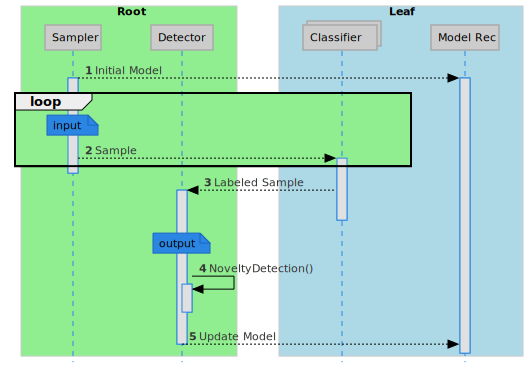
\includegraphics[width=\whencolumns{0.7}{1}\columnwidth,page=1]{figures/lifecycle.uml.svg.pdf}
    % \input{figures/lifecycle/lifecycle.latex}
  }
  \caption{\mfog life line overview.}
  \label{fig:mfog-mpi-life}
\end{figure}

The Sink Module was also build following reference techniques like
multi-class confusion matrix with label-class association
\cite{Faria2016minas}
to extract classification quality metrics.


% ------------------------------------------------------------------------------
\section{Experiments and Results}
\label{sec:experiments}

% Hermes Sugestão:
% Aiming to evaluate ... what we want evaluate (ex: the distributed novelty
% detection ...) we implemented an experimental scenario composed of ... three
% dedicated Raspberry Pi 3 connected by a 100 Gbps
% Ethernet switch to simulate an IoT network with constrained resources ...
% In this scenario a trafic genenrator reproduces the network traffic of the
% data set ... describe the data set. The load generator does bla bla bla ... The

Aiming to evaluate our proposal for the effects of distributed novelty detection
in a \iot \nids scenario, we implemented an experimental setup, composed of three Raspberry Pi 3 model B single board
computers connected via Ethernet Switch. The idea was to create a simple cluster simulating an
\iot network with constrained resources at the edge of the network.
This cluster stored all source code, binaries (compiled and linked in place) and
% data sets, being accessed via our laboratory network over Secure Shell (SSH).
data sets.
In our setup, the data set is stored in the root's node SD card and is read for
each experiment.
All experiments were executed in this cluster for isolation of otherwise
unforeseen variations and for safe software comparison with constant hardware.

The data set used is the December 2015 segment of
Kyoto 2006+ data set\footnote{Available at \url{http://www.takakura.com/Kyoto\_data/}.}
(Traffic Data from Kyoto University's Honeypots) \cite{Song2011}
containing $7\:865\:245$ samples.
From the original data set, we filtered only samples associated with normal traffic
or known attack types identified by existing \nids, and attack types with more
than $10\:000$ samples for significance, as previously done by
\cite{Cassales2019a}.
% , this removes 46,390 instances. TODO: revisar, pois 7M != 700K.
The remaining samples then were normalized so each feature value space (e.g., IP
Address, Duration, Service) is translated to the Real interval $[0, 1]$.

% Hermes: 72,000 em ingles usar a “,“ como separador de milhar
% SI/ISO 31-0 standard,
% Numbers consisting of long sequences of digits can be made more readable by
% separating them into groups, preferably groups of three, separated by a small
% space. For this reason, ISO 31-0 specifies that such groups of digits should
% never be separated by a comma or point, as these are reserved for use as the
% decimal sign. For example, one million (1000000) may be written as 1 000 000.

The resulting derived data set is then stored in two sets,
training set and test set, using the holdout technique.
However, for the training set we filter in only normal class
resulting in $72\:000$ instances.
For the test set we use $653\:457$ instances with
$206\:278$ instances with ``$N$'' (normal) class and
$447\:179$ instances with ``$A$'' (attack) class.
Note that this choice results in possible overfitting for the normal class and,
under-fitting for the attack class as the system first needs to detect a novel class and
then add it to the model.

% Count per class
%            id
% class        
% A      447179
% N      206278

% \begin{quote}
%   For the experiments, we used the Kyoto 2006+ data set
%   which contains data collected from 2006 to December 2015.
%   We selected examples from one month, December, 2015. Only the examples of known
%   attack types and known IDS alert code with a minimum of 10,000 occurrences (for
%   significance) were considered. The offline training was performed with 72,000
%   examples (i.e., 10\% of the data set) using the holdout technique.
%   \cite{Cassales2019a}
% \end{quote}

% \begin{highlight}
% O que quer testar com os experimentos.
% \begin{itemize}
%   \item Tese: Mostrar que detecção por novidade e classificação continua viável em fog.
%   \item Seria inviável por conta do atraso de distribuição de modelo e,
%   \item limitação pelo hardware pequeno.
%   \item MFOG: Um Agregador Regional, instalado na FOG, que observa a rede local.
% \end{itemize}

% Como realizou (cenário, rpi, setup, coleta de métricas).

% Quais resultados obteve.

% Como interpretar os resultados.
% \end{highlight}

% \hl{BEGIN Oritações de leitura das métricas e visualizações.}

\subsection{Measurements and Visualizations}

We have used two types of evaluation measurements for each experiment:
a measure of the full experiment execution time
% extracted by using \emph{GNU Time 1.9} measuring 
and, a set of qualitative measurements extracted by a Python script.

% Our script computed the
Our evaluation script was build following reference techniques like
multi-class confusion matrix with label-class association \cite{Faria2016minas}
to extract classification quality measurements.
This script takes two inputs, the test data set and the captured output stream,
and outputs the confusion matrix, label-class association,
final quality summary with:
\emph{Hits} (true positive), \emph{Misses} (Err), \emph{Unknowns} (UnkR); and
stream visualization chart with per example instance summary with novelty label markers.
% 
% For clarity, it is necessary to detail how to interpret and compare each measure,
% as for some it is trivial but others are not so much.

In the confusion matrix $M = m_{ij} \in \mathbb{N} ^{c \times{} l}$, computed by
our evaluation script, each row denotes % one of the data sets original 
the actual class $c$ and each column denotes the predicted label $l$ present in
the captured output stream.
Thus, each cell $M_{c, l}$ contains the count of examples from the test data set
of class $c$ found in the output stream with the label $l$ assigned by the under
evaluation experiment.

For the data set under use, original classes are $c \in \{N, A\}$, and for the
labels we have the training class
\emph{``N''}, \emph{unknown} label \emph{``-''} and the novelties $i \in
\mathbb{N}$ so $l \in \{N, -\} \cup \mathbb{N}$.

Added to the original confusion matrix $M$ are the rows \emph{Assigned} and
\emph{Hits}.
\emph{Assigned} row represents which original class $c$ (or if \emph{unknown},
\emph{``-''}) the label $l$ is assigned to, this is computed by using the
original class if $c = l$ or by associated novelty label to original class as
described in \cite{DeFaria2015evaluation} section 4.1
(class from where the most samples came from).
\emph{Hits} row shows the true positive count for each label $l$
with assigned class $c$, being the same value as cell $M_{c, l}$.
% computed by coping the value of the 
%  where the label is the same
% and the class $c$ is the value in the above \emph{Assigned} row.
The \emph{Hits} row is also used to compute the overall true positive
in the summary table and stream visualization chart.
% accuracy.
One complete matrix is shown in Tab. \ref{tab:java-matrix}.

% \begin{table*}[htb]\begin{center}
%   \caption{Reference implementation: Confusion Matrix and Qualitative Metrics}
%   \input{experiments/revised-java.log.tex}
%   \label{tab:java-matrix}
% \end{center}\end{table*}

\begin{table*}[htb]
\caption{Confusion Matrices and Qualitative measurements}
\label{tab:confusion-matrixes-ref-serial}
\begin{subtable}[h]{\textwidth}\begin{center}
    \caption{Reference implementation}
    \input{experiments/revised-java.log.tex}
    \label{tab:java-matrix}
\end{center}\end{subtable}
\begin{subtable}[h]{\textwidth}\begin{center}
    \whencolumns{}{\vspace{5mm}}
    \caption{Serial implementation}
    \input{experiments/online-nd.log.tex}
    \label{tab:libc-matrix}
    \whencolumns{}{\vspace{5mm}}
\end{center}\end{subtable}
\begin{subtable}[h]{0.5\textwidth}\begin{center}
  \caption{Parallel single-node}
  \input{experiments/tmi-base.log.tex}
  \label{tab:single-node-matrix}
\end{center}\end{subtable}
\begin{subtable}[h]{0.5\textwidth}\begin{center}
  \caption{Parallel multi-node}
  \input{experiments/tmi-n12.log.tex}
  \label{tab:multi-node-matrix}
\end{center}\end{subtable}
\end{table*}

For the measurements summary table, six measurements from two sources are displayed. Three
measures \emph{Hits}, \emph{Unknowns} and \emph{Misses} represented as ratio of
the captured output stream, extracted from the evaluation python program,
computed as follows:
\emph{Hits} (true positive rate) is the sum of the \emph{Hits} row in the
extended confusion matrix;
\emph{Unknowns} is the count of examples in the captured output stream marked
with the \emph{unknown} label (\emph{``-''});
\emph{Misses} is the count of all examples in the captured output stream marked
with a label distinct from the \emph{Assigned} original class and are not marked
as unknown.

Furthermore in the measurement summary table, \emph{Time}, \emph{System} and \emph{Elapsed}
 represented in seconds, are extracted from \emph{GNU Time 1.9}.
\emph{Time} is the amount of CPU seconds expended in user-mode
(indicates time used doing CPU intensive computing, e.g., math);
\emph{System} is the amount of CPU seconds expended in kernel-mode
(for our case, it indicates time doing input or output);
\emph{Elapsed} is the real-world (wall clock) elapsed time and
indicates how long the program took to complete.
The lower the times, the better.
Our four main experiments are shown in Tab. \ref{tab:exper-summary}.

Lastly, the stream visualization chart shows the summary quality measurement
(\emph{Hits}, \emph{Unknowns}, \emph{Misses})
computed for each example in the captured output stream.
This summary is computed for each example, but it uses the \emph{Assigned} row
computed previously to evaluate \emph{Hits}; the other measurements are derived as
described before.
The Horizontal axis (x, domain) plots the index of the example and the
vertical axis (y, image) shows the measurement computed until that example index on the captured
output stream.

Adding to the stream visualization chart, novelty label markers are represented
as vertical lines indicating \emph{when} in the captured output stream a new
label first appeared.
Some of the novelty label markers include the label itself ($l \in \mathbb{N}$)
for reference (showing every label would turn this feature unreadable due
to overlapping).
Figure \ref{fig:visualization} shows complete stream visualization charts.

\begin{figure*}[hbt]
  \centerline{
    \begin{subfigure}{.5\textwidth}
      \centering
      % \includegraphics[trim={0.2cm 0 1.9mm 0},clip,width=\linewidth]{experiments/revised-java.log.png}
      \includegraphics[width=\linewidth]{experiments/revised-java.log.png}
      \caption{Reference Implementation}
      \label{fig:validation-sub-java}
    \end{subfigure}
    \begin{subfigure}{.5\textwidth}
      \centering
      \includegraphics[width=\linewidth]{experiments/online-nd.log.png}
      \caption{Serial Implementation}
      \label{fig:validation-sub-serial}
    \end{subfigure}
  }
  \whencolumns{}{\vspace{5mm}}
  \centerline{
    \begin{subfigure}{.5\textwidth}
      \centering
      \includegraphics[width=\linewidth]{experiments/tmi-base.log.png}
      \caption{Parallel single-node}
      \label{fig:cluster-sub-single}
    \end{subfigure}
    \begin{subfigure}{.5\textwidth}
      \centering
      \includegraphics[width=\linewidth]{experiments/tmi-n12.log.png}
      \caption{Parallel multi-node}
      \label{fig:cluster-sub-multi}
    \end{subfigure}
  }
  % \caption{Validation Comparison: Stream hits and novelties visualization}
  % \label{fig:validation-java-serial}
  \caption{Stream hits and novelties visualization.}
  \label{fig:visualization}
\end{figure*}

% \hl{END Oritações de leitura das métricas e visualizações.}

% \FloatBarrier
\subsection{Discussion}

Four main experiments are presented for discussion:
(\emph{a}) reference implementation of Minas (\refminas) \cite{Faria2016minas};
(\emph{b}) new implementation in serial mode;
(\emph{c}) new implementation in single-node, multi-task mode and
(\emph{d}) new implementation in multi-node, multi-task mode.
Each experiment uses the adequate binary executable, initial model
(or training set for the reference implementation) and test set
to compute a resulting output stream which is stored for qualitative evaluation.
The summary of all four experiments is shown in Table \ref{tab:exper-summary}.

\begin{table*}[hbt]
\begin{center}
  \caption{Collected Measures Summary.}
  \label{tab:exper-summary}
  \input{experiments/summary.tex}
\end{center}
\end{table*}

The comparison of the first two experiments (\emph{a} and \emph{b}) provides a
validation for our implementation, while the latter three (\emph{b}, \emph{c}
and \emph{d}) serve as showcase for the effects of distribution.

As stated, to validate our implementation we have compared it to \refminas
(the original \minas companion implementation), so we extracted the same measurements
using same process for both \emph{a} and \emph{b}, which can be viewed in
Tables \ref{tab:java-matrix}, \ref{tab:libc-matrix} and for ease of comparison
in Table \ref{tab:exper-summary} the summary can be compared side by side.

In general, the observed classification quality measurements are very similar,
and only diverge slightly where \emph{a} has more \emph{Hits} and \emph{Misses}
whereas \emph{b} shifted those to \emph{Unknowns}.
This phenomenon was watched very closely during development and we found that it was due to
small changes to \minas parameters, \minas internals like K-means ordering,
cluster edge inclusion and cluster radius formula as stated in
Subsection \ref{sec:implementation}.

As for the time measurements in Table \ref{tab:exper-summary}
our implementation used less time to analyze the test data set.
This is mostly due to 
the stop condition
on the internal K-means algorithm; while \refminas uses a fixed iteration
limit of $100$, our implementations adds the ``no improvement'' check
and stops earlier in most cases, which in turn reduces the time taken
on the \emph{NoveltyDetection} function.
There are also small optimizations on the \emph{nearestCluster} function
(minimal distance from sample to cluster center in the set)
affecting the \emph{classifier} task and \emph{NoveltyDetection} function.
One can also note that \refminas time in \emph{a} includes the Offline phase while our
implementation runs it once and reuses the initial model for \emph{b}, \emph{c}
and \emph{d}. In the table the offline time this is shown as a separate column.

As for the effects of running the classification processes on the small devices as MPI nodes with our implementation, we observe
an increase of time when we go from $2$ to $4$ instances in a single node
(\emph{b} and \emph{c} respectively), hinting that our choice of load
distribution is not as effective as we expected.
Further experiments were conducted with the number of instances varying from $1$ (serial) to
$12$ (3 nodes with 4 CPUs each), but that caused no impact on the true positive rate (\emph{Hits}) and elapsed time.
More detailed time measurements can be seen in Figure \ref{fig:speedup},
where we observe near constant time for \emph{elapsed} (near $100s$),
the \emph{system} increases gradually while \emph{user} decreases at the same rate.
We interpret this behavior as a display of potential for gains using a better
load balancing than our choice of round-robin such as micro-batching for better
compute-to-communication ratio (CCR).
% legal!
In general, Figure \ref{fig:speedup} shows no speedup but also no penalty for
scaling to more than $4$ instances.

% \st{we have to say it is pretty shitty because of our choice of distribution 
% using round-robin, use some load balancing and micro-batching for better results.}

% Tempo gasto com distribuição e tempo gasto com processamento mostra que é viável.

% relação $p/n$ 

% relação do tempo comm / tempo processing
% coom time / processing time does not inhibit the use of our aproach.
% CCR

% compute-to-communication ratio (CCR) indicates that our approach is viable 

% compute-to-communication ratio (CCR).

\begin{figure}[hbt]
  \centering
  % \includegraphics[width=\linewidth]{experiments/speedup-clean.png}
  \includegraphics[width=\whencolumns{0.6}{1}\linewidth,page=1]{experiments/speedup-clean.pdf}
  \caption{Time measurements per added instance.}
  \label{fig:speedup}
\end{figure}

Nevertheless, we can also show the effects of delay in the
Classify, Novelty Detection, Model Update and Classify feedback loop.
Comparing \emph{b} and \emph{c} we observe a reduction in Novelty labels
on the Confusion Matrix (tabs. \ref{tab:libc-matrix} and \ref{tab:single-node-matrix})
from $10$ to $4$.
The same effect is observed on the stream visualization (figs.
\ref{fig:validation-sub-serial} and \ref{fig:cluster-sub-single}) where our
serial implementation has fewer novelty markers, and they appear later, but the
measures keep the same ``shape''.
Comparing \emph{c} and \emph{d} the difference is even smaller,
(figs. \ref{fig:validation-sub-serial} and \ref{fig:cluster-sub-single})
as they both suffer the expected delay in the feedback loop.

% \todo{discutir o delay de 80k entre etiqueta 0 em serial vs node}

% When observing the stream visualization on figure \ref{fig:cluster-sub-multi}

% \begin{table*}[htb]
% \caption{Confusion Matrix and Qualitative measures for MPI Clusters.}
% \label{tab:confusion-matrixes-single-multi}
% \begin{subtable}[h]{0.5\textwidth}\begin{center}
%     \caption{Parallel single-node}
%     \input{experiments/tmi-base.log.tex}
%     \label{tab:single-node-matrix}
% \end{center}\end{subtable}
% \begin{subtable}[h]{0.5\textwidth}\begin{center}
%     \caption{Parallel multi-node}
%     \input{experiments/tmi-n12.log.tex}
%     \label{tab:multi-node-matrix}
% \end{center}\end{subtable}
% \end{table*}

% 22.40 user	0.02 system	0:22.48 elapsed

% \begin{table*}[htb]\begin{center}
%   \caption{Serial implementation: Confusion Matrix and Qualitative Metrics}
%   \input{experiments/online-nd.log.tex}
%   \label{tab:libc-matrix}
% \end{center}\end{table*}

% \begin{figure*}[htb]
%   \centerline{
%     \begin{subfigure}{.5\textwidth}
%       \centering
%       \includegraphics[width=\linewidth]{experiments/tmi-base.log.png}
%       \caption{Parallel single-node}
%       \label{fig:cluster-sub-single}
%     \end{subfigure}
%     \begin{subfigure}{.5\textwidth}
%       \centering
%       \includegraphics[width=\linewidth]{experiments/tmi-n12.log.png}
%       \caption{Parallel multi-node}
%       \label{fig:cluster-sub-multi}
%     \end{subfigure}
%     % \begin{subfigure}{.5\textwidth}
%     %   \centering
%     %   \includegraphics[width=\linewidth]{experiments/speedup-clean.png}
%     %   \caption{Time measurements per added instance}
%     %   \label{fig:cluster-sub-multi}
%     % \end{subfigure}
%   }
%   \caption{Parallelism Comparison: Stream hits and novelties visualization}
%   \label{fig:cluster}
% \end{figure*}


% \begin{table}[htb]\begin{center}
%   \caption{Parallel single-node: Confusion Matrix and Qualitative Metrics}
%   \input{experiments/tmi-base.log.tex}
%   \label{tab:single-node-matrix}
% \end{center}\end{table}

% \setcounter{MaxMatrixCols}{20}
% \begin{table*}[htb]
  %   \begin{center}
    %     \caption{Reference implementation: Confusion Matrix and Qualitative Metrics}
    %     \begin{math}\begin{pmatrix}
      %       - & N & 1 & 2 & 3 & 4 & 5 & 6 & 7 & 8 & 9 & 10 & 11 & 12
%     \end{pmatrix}\end{math}
%     \begin{math}\begin{pmatrix}
%     3774 &  438750 &  123 &  145 &  368 &  8 &  52 &  165 &    1 &  1046 &  161 &  2489 &   71 &  26 \\
%     8206 &  193030 &    0 &   79 &   44 &  0 &   0 &    0 &  229 &   181 &  154 &  4066 &  289 &   0
%     \end{pmatrix}\end{math}
%     \begin{math}\begin{pmatrix}
%       - &       N &    A &    A &    A &  A &   A &    A &    N &     A &    A &     N &    N &   A \\
%       0 &  193030 &  123 &  145 &  368 &  8 &  52 &  165 &  229 &  1046 &  161 &  4066 &  289 &  26 
%     \end{pmatrix}\end{math}
%     \label{math-tab}
%   \end{center}
% \end{table*}

% \begin{figure*}
%   \centering
%   \centerline{
%     \includegraphics[width=0.45\textwidth]{../experiments/revised-java.log.png}
%     \includegraphics[width=0.45\textwidth]{../experiments/revised-java.log.png}
%   }
%   \\
%   \centerline{
%     \includegraphics[width=0.45\textwidth]{../experiments/revised-java.log.png}
%     \includegraphics[width=0.45\textwidth]{../experiments/revised-java.log.png}
%   }
% \label{fig1} 
% \end{figure*}

% \begin{highlight}

% \end{highlight}



% ----------------------------------------------------------------------------------------------------------------------
\section{Conclusion {\color{red} Nao mexer por enquanto}} 
\label{sec:conclusion}

% ----------------------------------------------------------------------------------------------------------------------
\section*{Acknowledgment}

% The preferred spelling of the word ``acknowledgment'' in America is without an ``e'' after the ``g''.
% Avoid the stilted expression ``one of us (R. B. G.) thanks $\ldots$''.
% Instead, try ``R. B. G. thanks$\ldots$''.
% Put sponsor  acknowledgments in the unnumbered footnote on the first page.
The authors thank CNPq (Contract 167345/2018-4).
Hermes Senger also thanks CNPq (Contract 305032/2015-1) and FAPESP (Contract
2018/00452-2, and Contract 2015/24461-2) for their support.


\bibliographystyle{splncs04.bst}
\bibliography{99-refs-ISCC}
\end{document}
